\section{Predictions and Observations}

Observed data (36.1 \ifb) and predicted SM backgrounds event yields 
are compared in Fig.~\ref{fig:results_datamc_rpc} for signal regions addressing $R$-parity-conserving signal scenarios, 
for events satisfying the SR requirements except the \met\ cut. Adjustments to the selections are made: 
\begin{itemize}
\item SRs involving an effective mass cut: it is relaxed 
together with the \met\ cut to avoid indirectly tightening requirements 
on the visible leptonic and hadronic contributions to \meff\ for low values of \met; 
the \meff\ requirement is therefore changed to:
$$
\meff > \left(m_\mathrm{eff}^\text{SR cut}\right) - \operatorname{max}\left[\left(E_\mathrm{T}^\text{miss, SR cut}\right)-\met,0\right]
$$
\item SRs involving a cut on the $\met/\meff$ ratio: it is relaxed together with the \met\ cut 
to allow populating the low \met\ tail of the distributions: 
$$
\frac{\met}{\meff} > \left(\frac{\met}{\meff}\right)^\text{SR cut}\times \frac{\met}{\left(E_\mathrm{T}^\text{miss, SR cut}\right)^\text{SR cut}}
$$
in addition, an upper cut on \meff\ is added. 
\end{itemize}

\begin{figure}[p!]
\centering
 \begin{subfigure}{0.42\textwidth}
 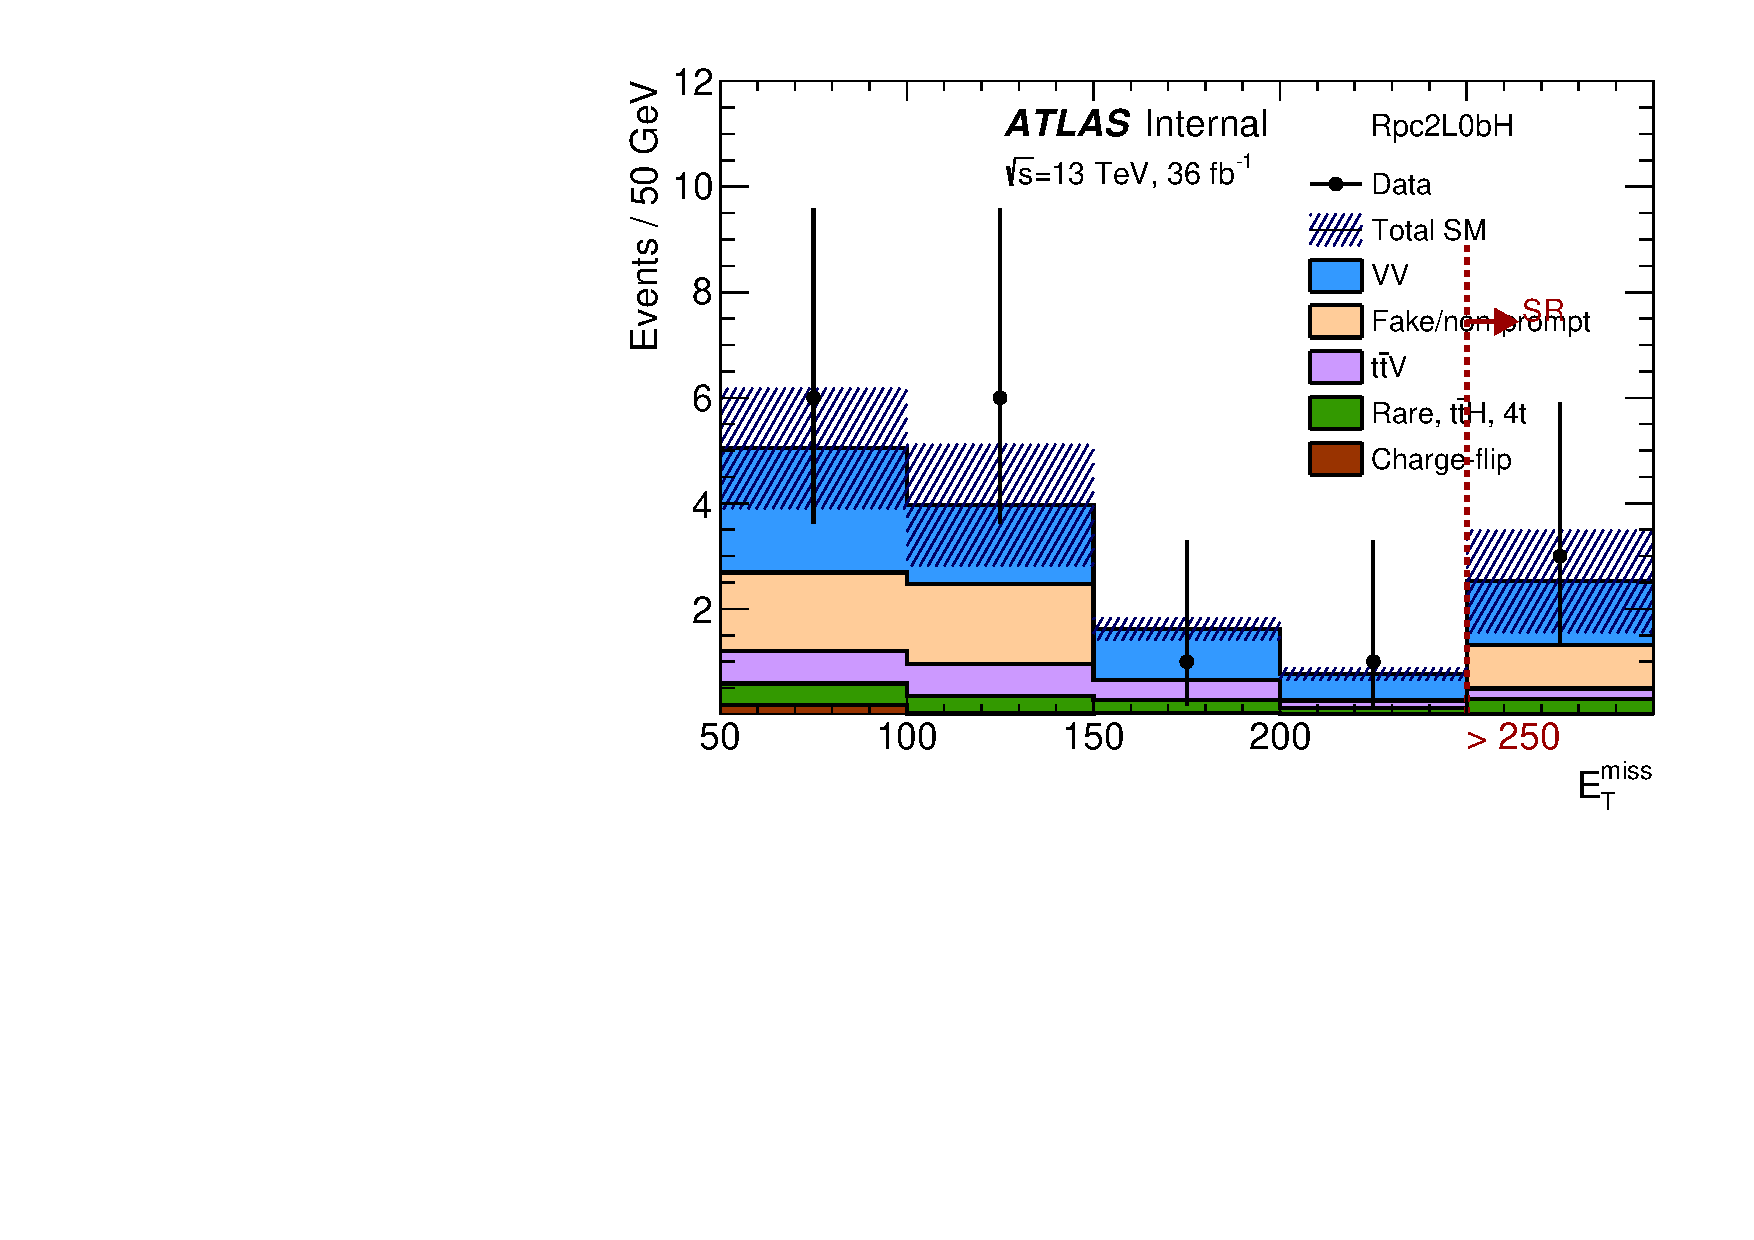
\includegraphics[width=\textwidth]{LooseRpc2L0bH.pdf}
 \subcaption{Rpc2L0bH before the \met\ requirement}
 \end{subfigure}
 \begin{subfigure}{0.42\textwidth}
 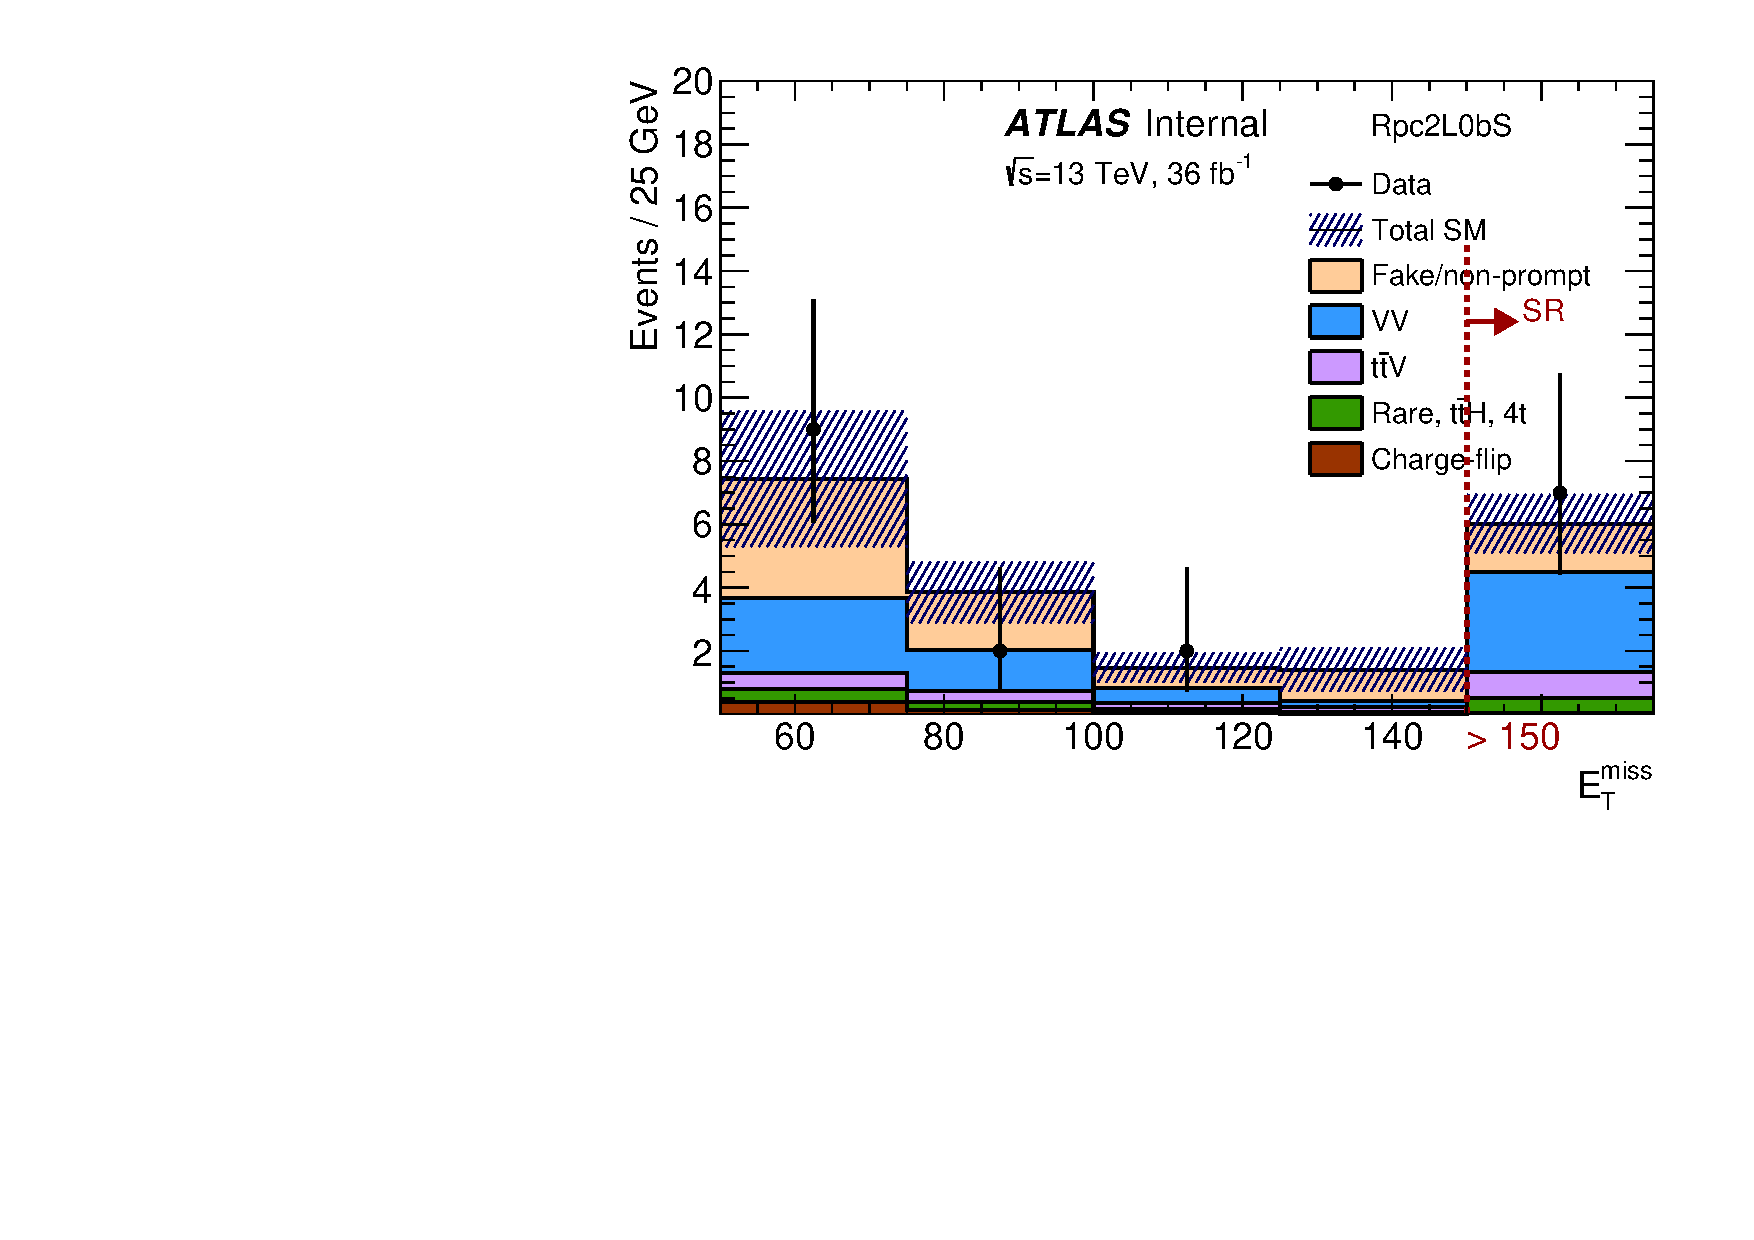
\includegraphics[width=\textwidth]{LooseRpc2L0bS.pdf}
 \subcaption{Rpc2L0bS before the \met\ requirement}
 \end{subfigure}
  \begin{subfigure}{0.42\textwidth}
 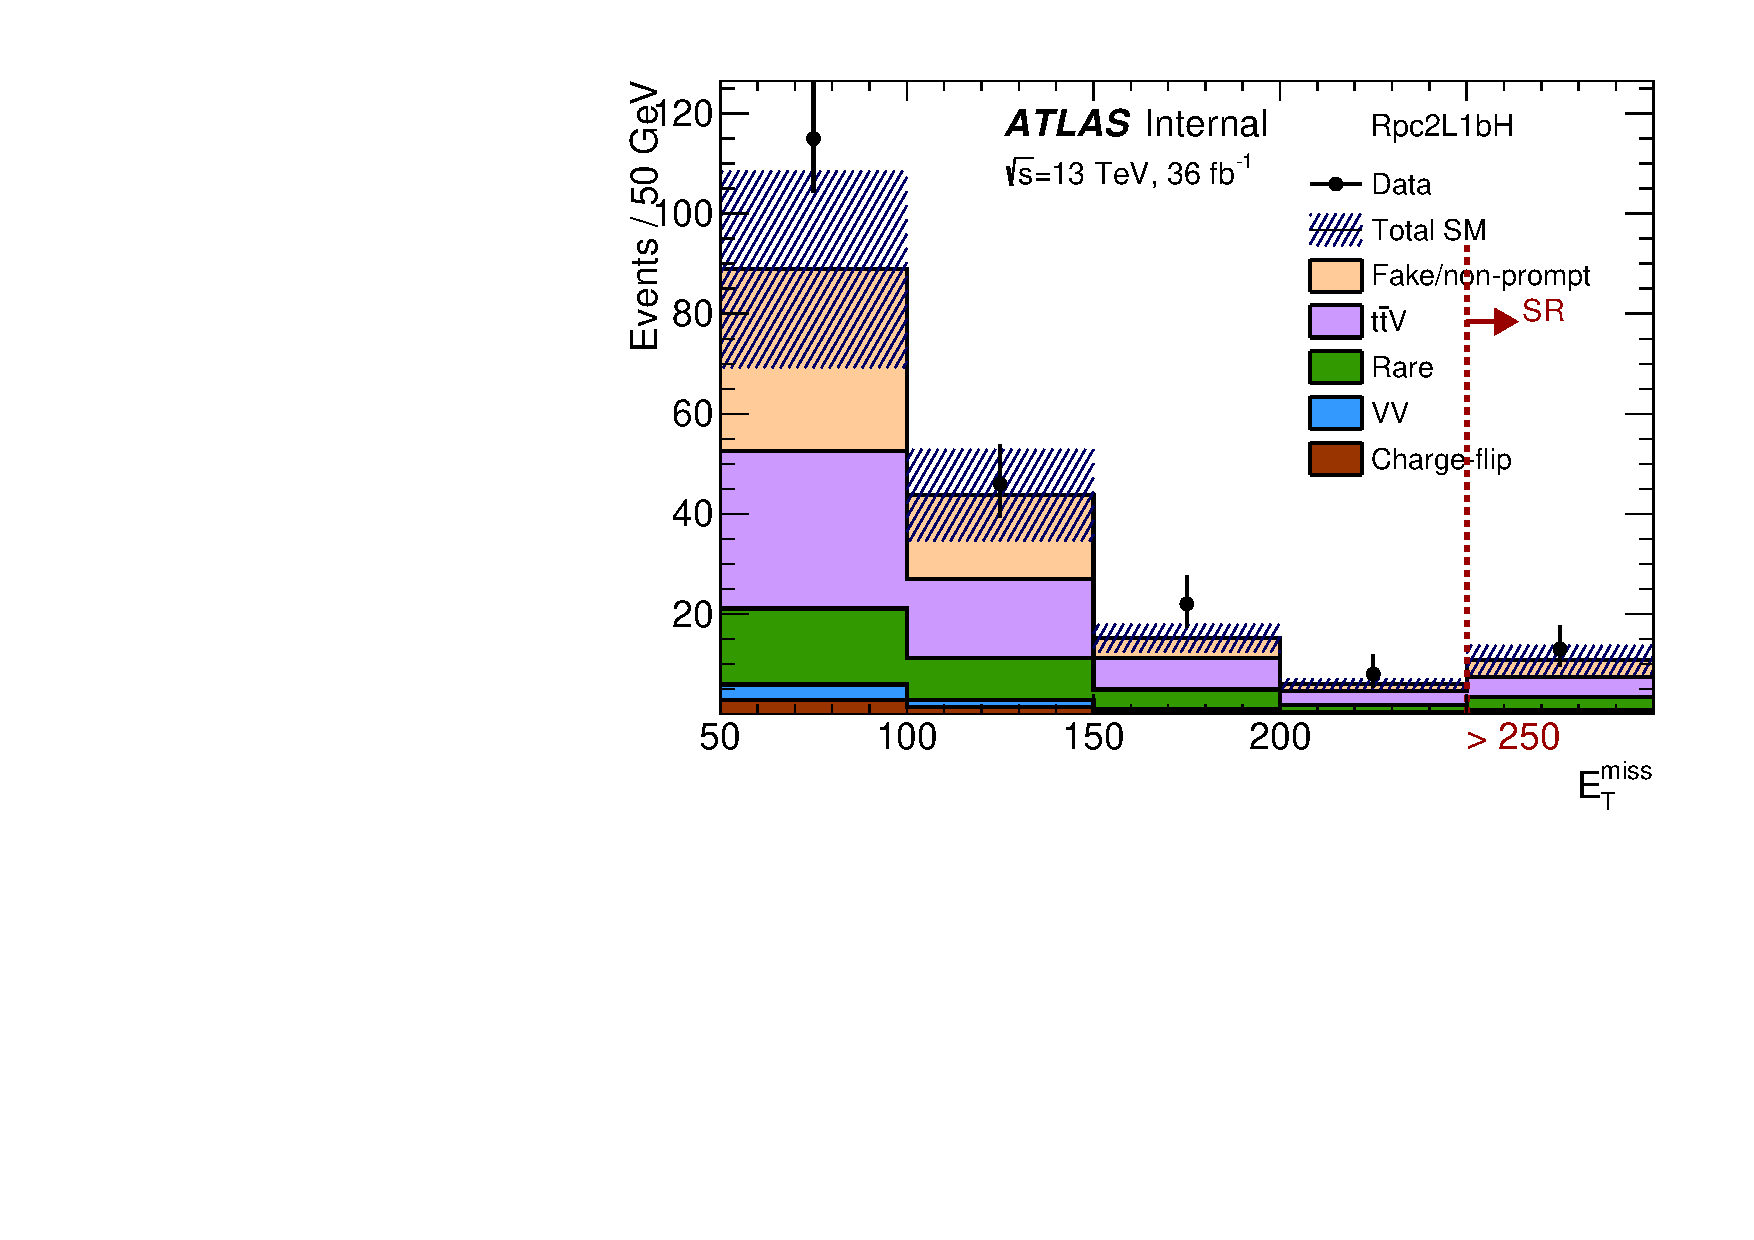
\includegraphics[width=\textwidth]{LooseRpc2L1bH.pdf}
 \subcaption{Rpc2L1bH before the \met\ requirement}
 \end{subfigure}
  \begin{subfigure}{0.42\textwidth}
 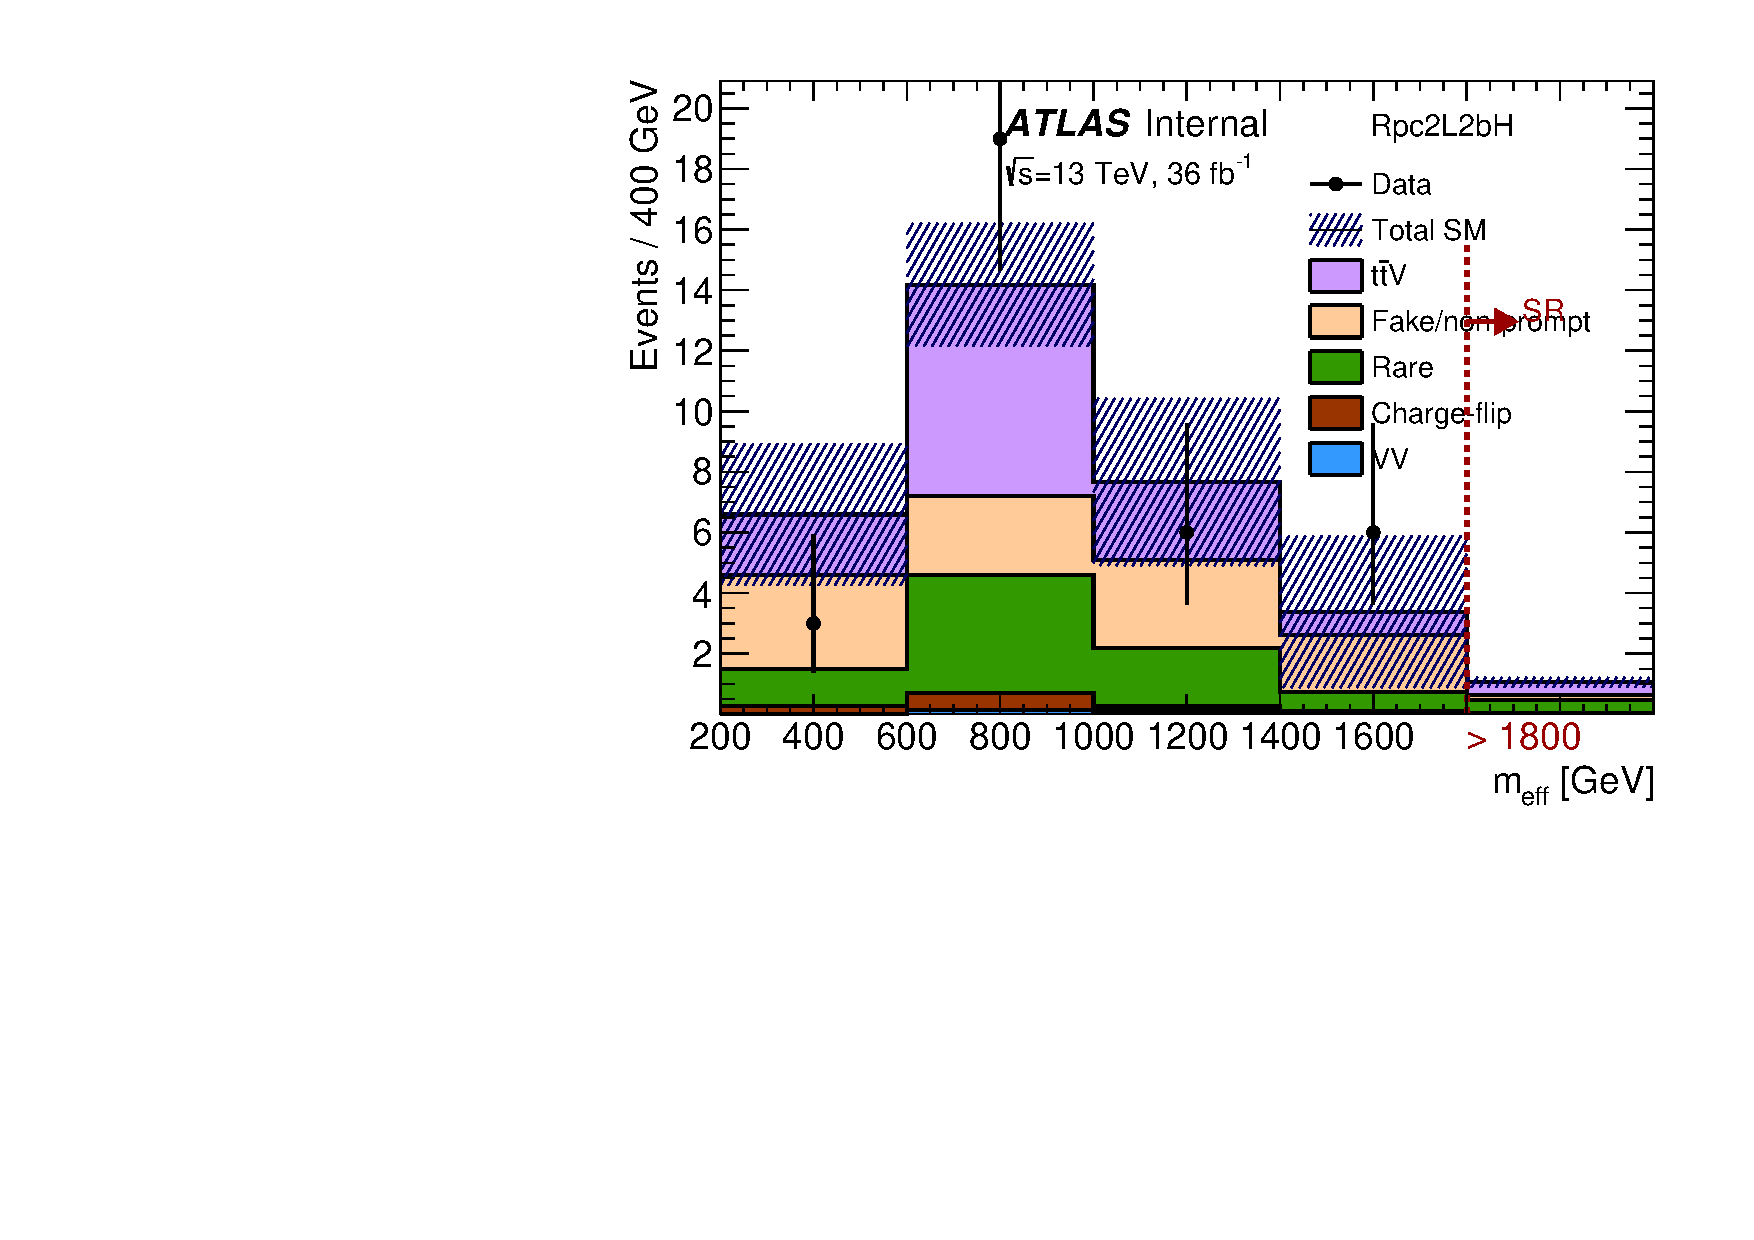
\includegraphics[width=\textwidth]{LooseRpc2L2bH.pdf}
 \subcaption{Rpc2L2bH before the \meff\ requirement}
 \end{subfigure}
   \caption{
Missing transverse momentum distributions for observed data and predicted backgrounds 
with the all the signal regions requirements, before the final \met\. 
The effective mass and/or $\met/\meff$ ratio cuts are also relaxed for \met\ values below the SR threshold (see text for details). 
The signal regions correspond to the last (inclusive) bins of the figures. 
The shaded area represents uncertainties on the total SM background estimate, 
which include all sources of statistical uncertainties, 
as well as the systematic uncertainties for fake lepton and charge-flip backgrounds. 
%The fake lepton background prediction is only coming from the matrix method here. 
%the contributions of statistical sources alone are highlighted by the light-shaded areas in the ratios plots. 
}
\label{fig:results_datamc_rpc}
\end{figure}


\begin{figure}[p!]
\centering
   \begin{subfigure}{0.42\textwidth}
 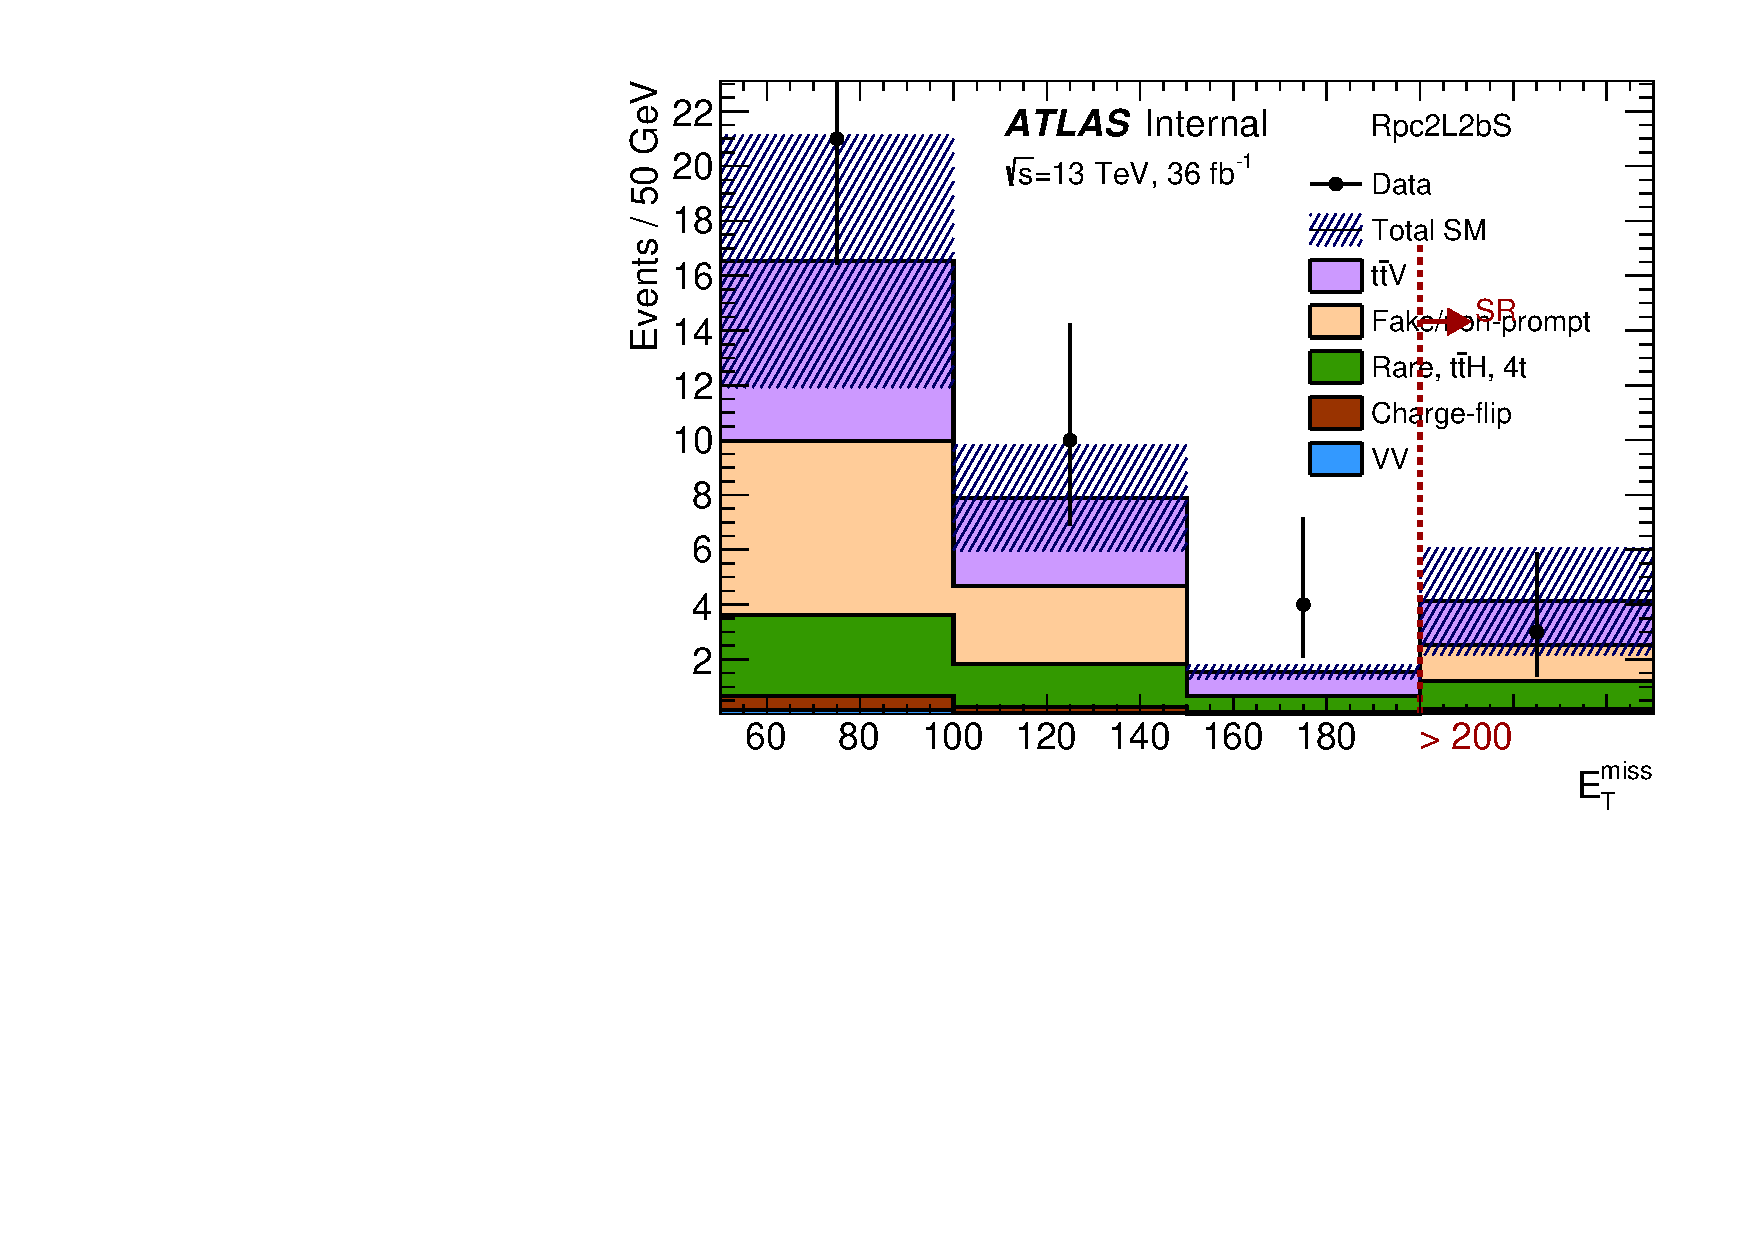
\includegraphics[width=\textwidth]{LooseRpc2L2bS.pdf}
 \subcaption{Rpc2L2bS before the \met\ requirement}
 \end{subfigure}
   \begin{subfigure}{0.42\textwidth}
 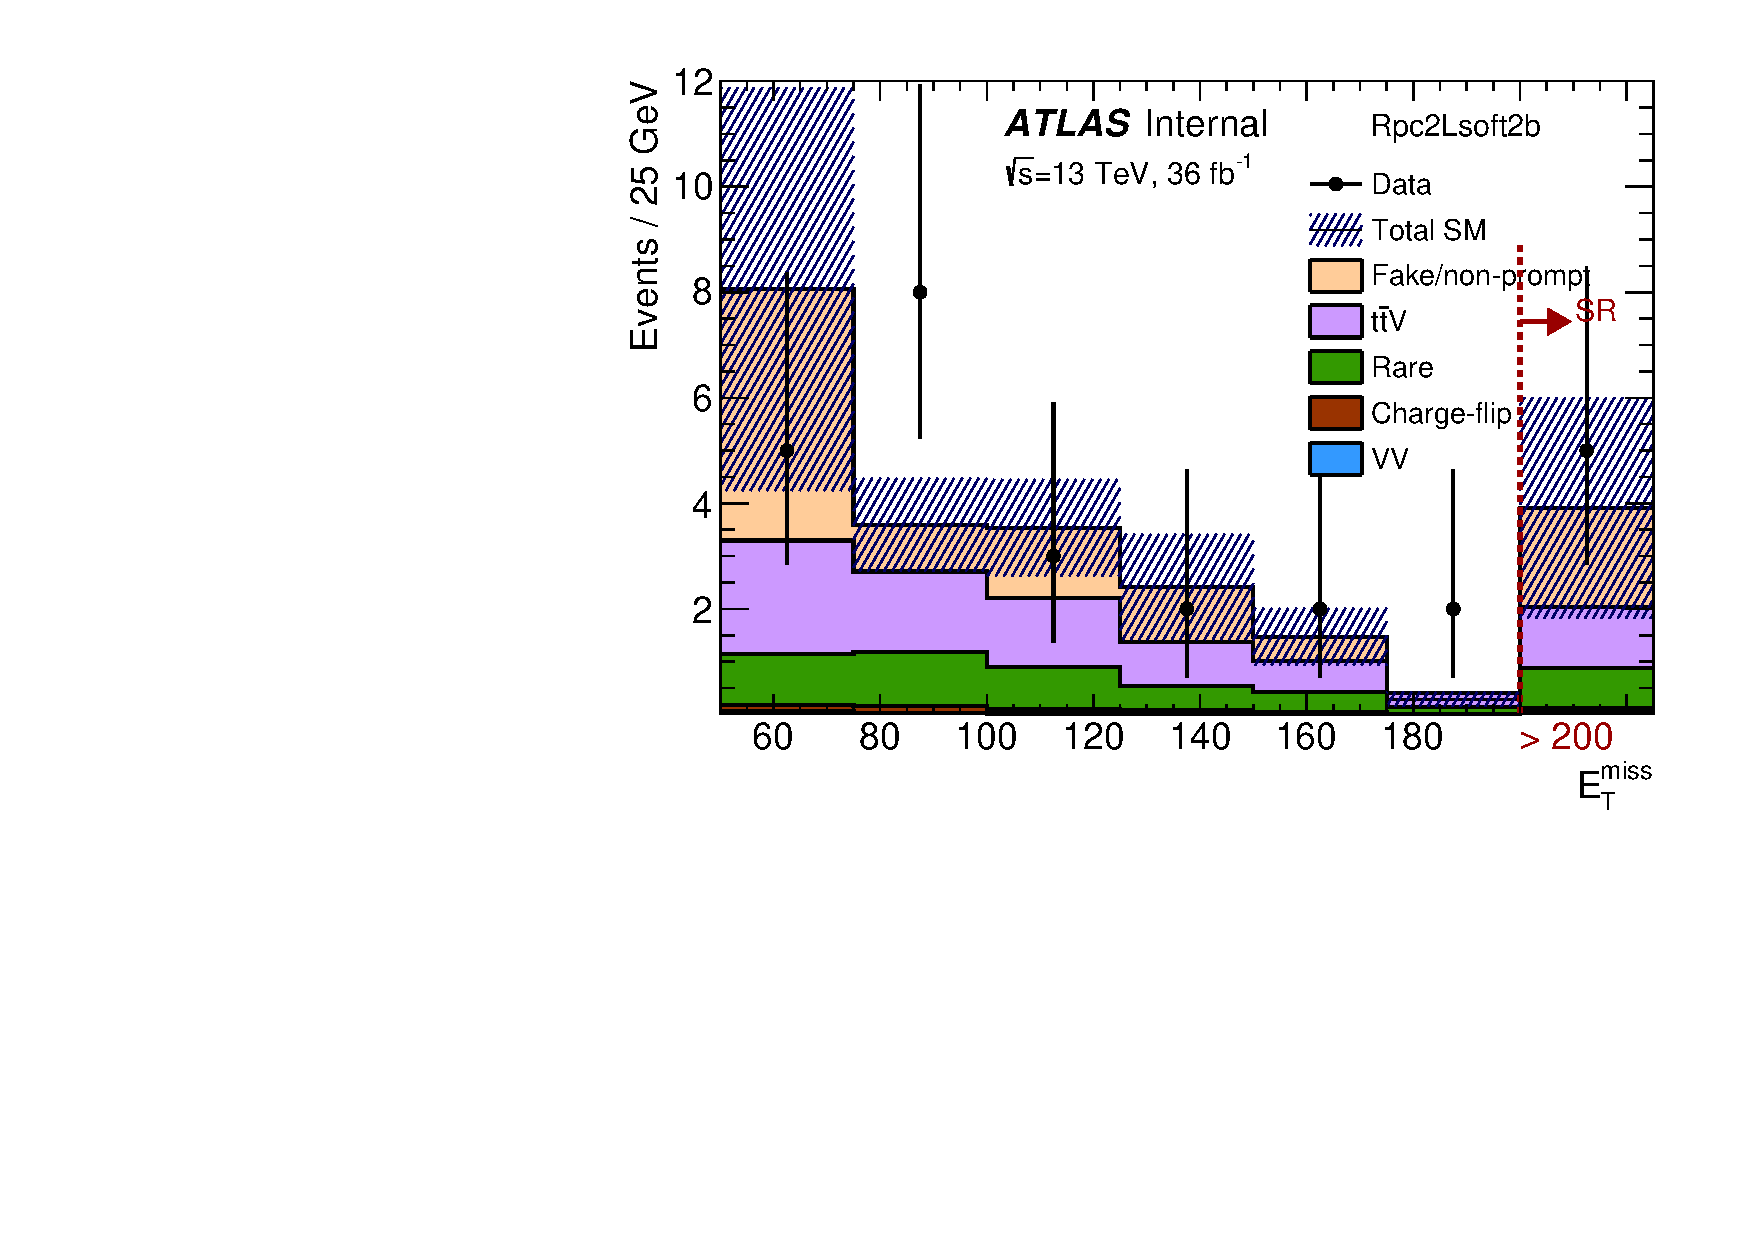
\includegraphics[width=\textwidth]{LooseRpc2Lsoft2b.pdf}
 \subcaption{Rpc2Lsoft2b before the \met\ requirement}
 \end{subfigure}
   \begin{subfigure}{0.42\textwidth}
 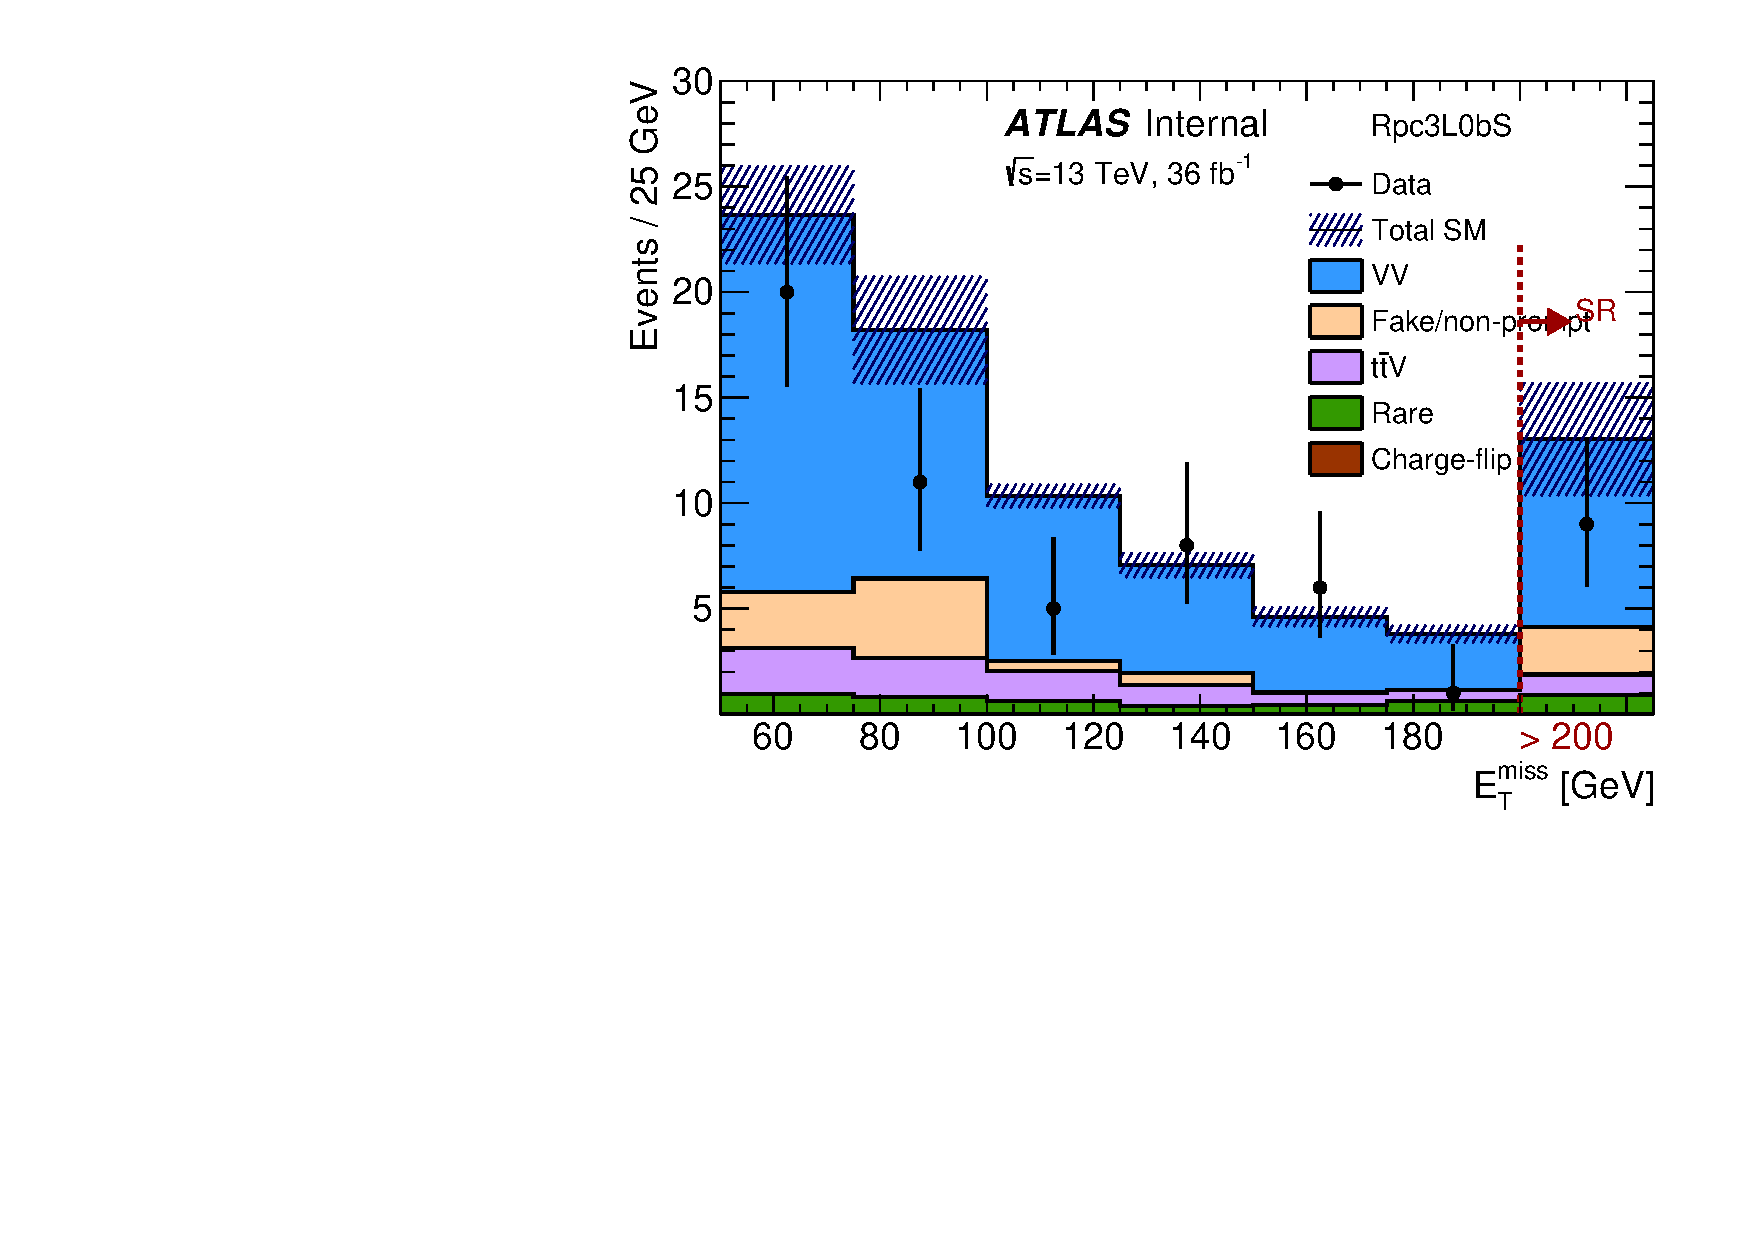
\includegraphics[width=\textwidth]{LooseRpc3L0bS.pdf}
 \subcaption{Rpc3L0bS before the \met\ requirement}
 \end{subfigure}
    \begin{subfigure}{0.42\textwidth}
 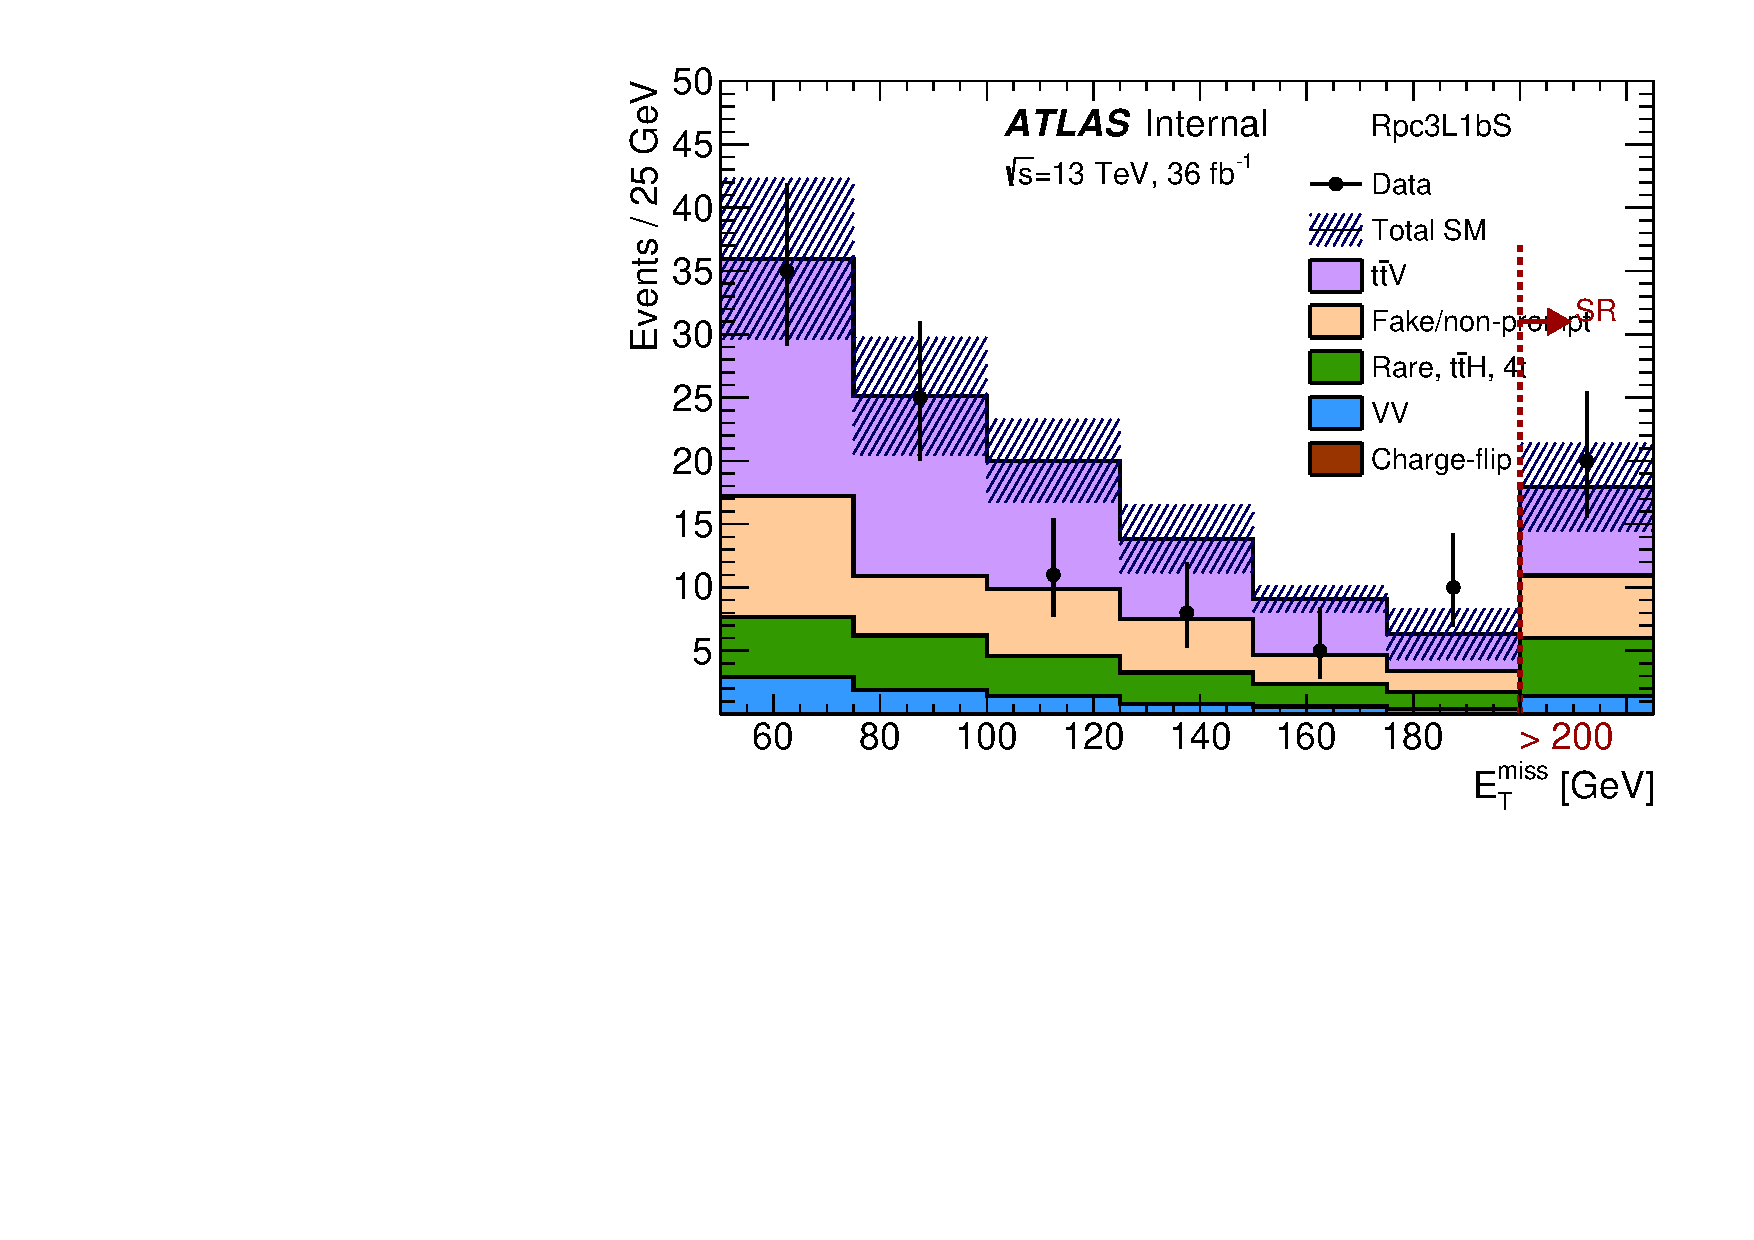
\includegraphics[width=\textwidth]{LooseRpc3L1bS.pdf}
 \subcaption{Rpc3L1bS before the \met\ requirement}
 \end{subfigure}
   \caption{
Missing transverse momentum distributions for observed data and predicted backgrounds 
with the all the signal regions requirements, before the final \met\. 
The effective mass and/or $\met/\meff$ ratio cuts are also relaxed for \met\ values below the SR threshold (see text for details). 
The signal regions correspond to the last (inclusive) bins of the figures. 
The shaded area represents uncertainties on the total SM background estimate, 
which include all sources of statistical uncertainties, 
as well as the systematic uncertainties for fake lepton and charge-flip backgrounds. 
}
\label{fig:results_datamc_rpc}
\end{figure}


Figure~\ref{fig:PlotSR} shows the event yields for data and the expected background contributions 
in all signal regions. Detailed information about the yields can be found in Table~\ref{tab:SR_yields}.
In all 13 SRs the number of observed data events is consistent with the expected background within the uncertainties. 
The contributions listed in the rare category are dominated by triboson, $tWZ$ and $\ttbar WW$ production.
The triboson processes generally dominate in the SRs with no $b$-jets, while $tWZ$ and $\ttbar WW$
dominate in the SRs with one and two $b$-jets, respectively. Contributions from $WH$, $ZH$, $tZ$ and $\ttbar t$ production 
never represent more than 20\% of the rare background.

\begin{figure}[t]
\begin{center}
\begin{subfigure}[t]{0.98\textwidth}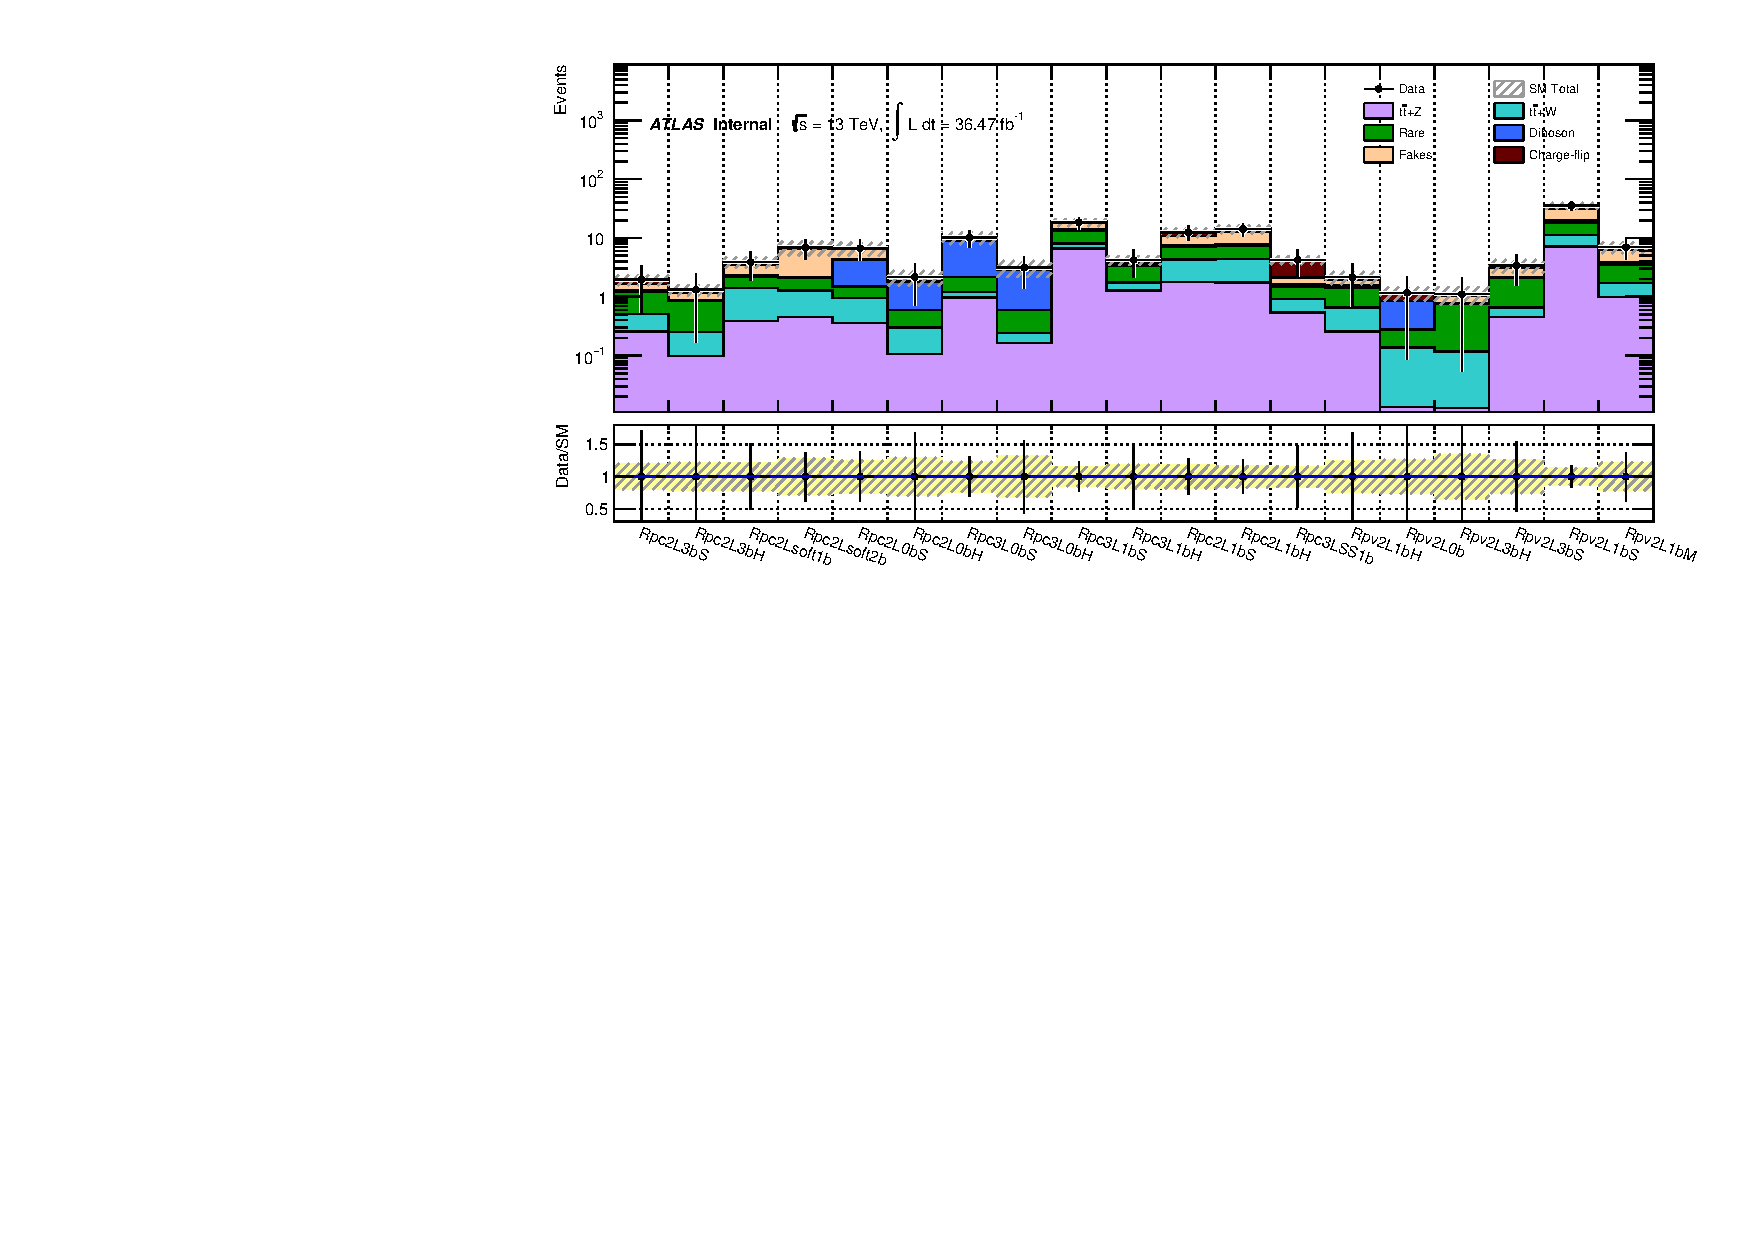
\includegraphics[width=\textwidth]{SRsummary}\caption{}\label{fig:Results_SRSum}\end{subfigure}
\begin{subfigure}[t]{1.08\textwidth}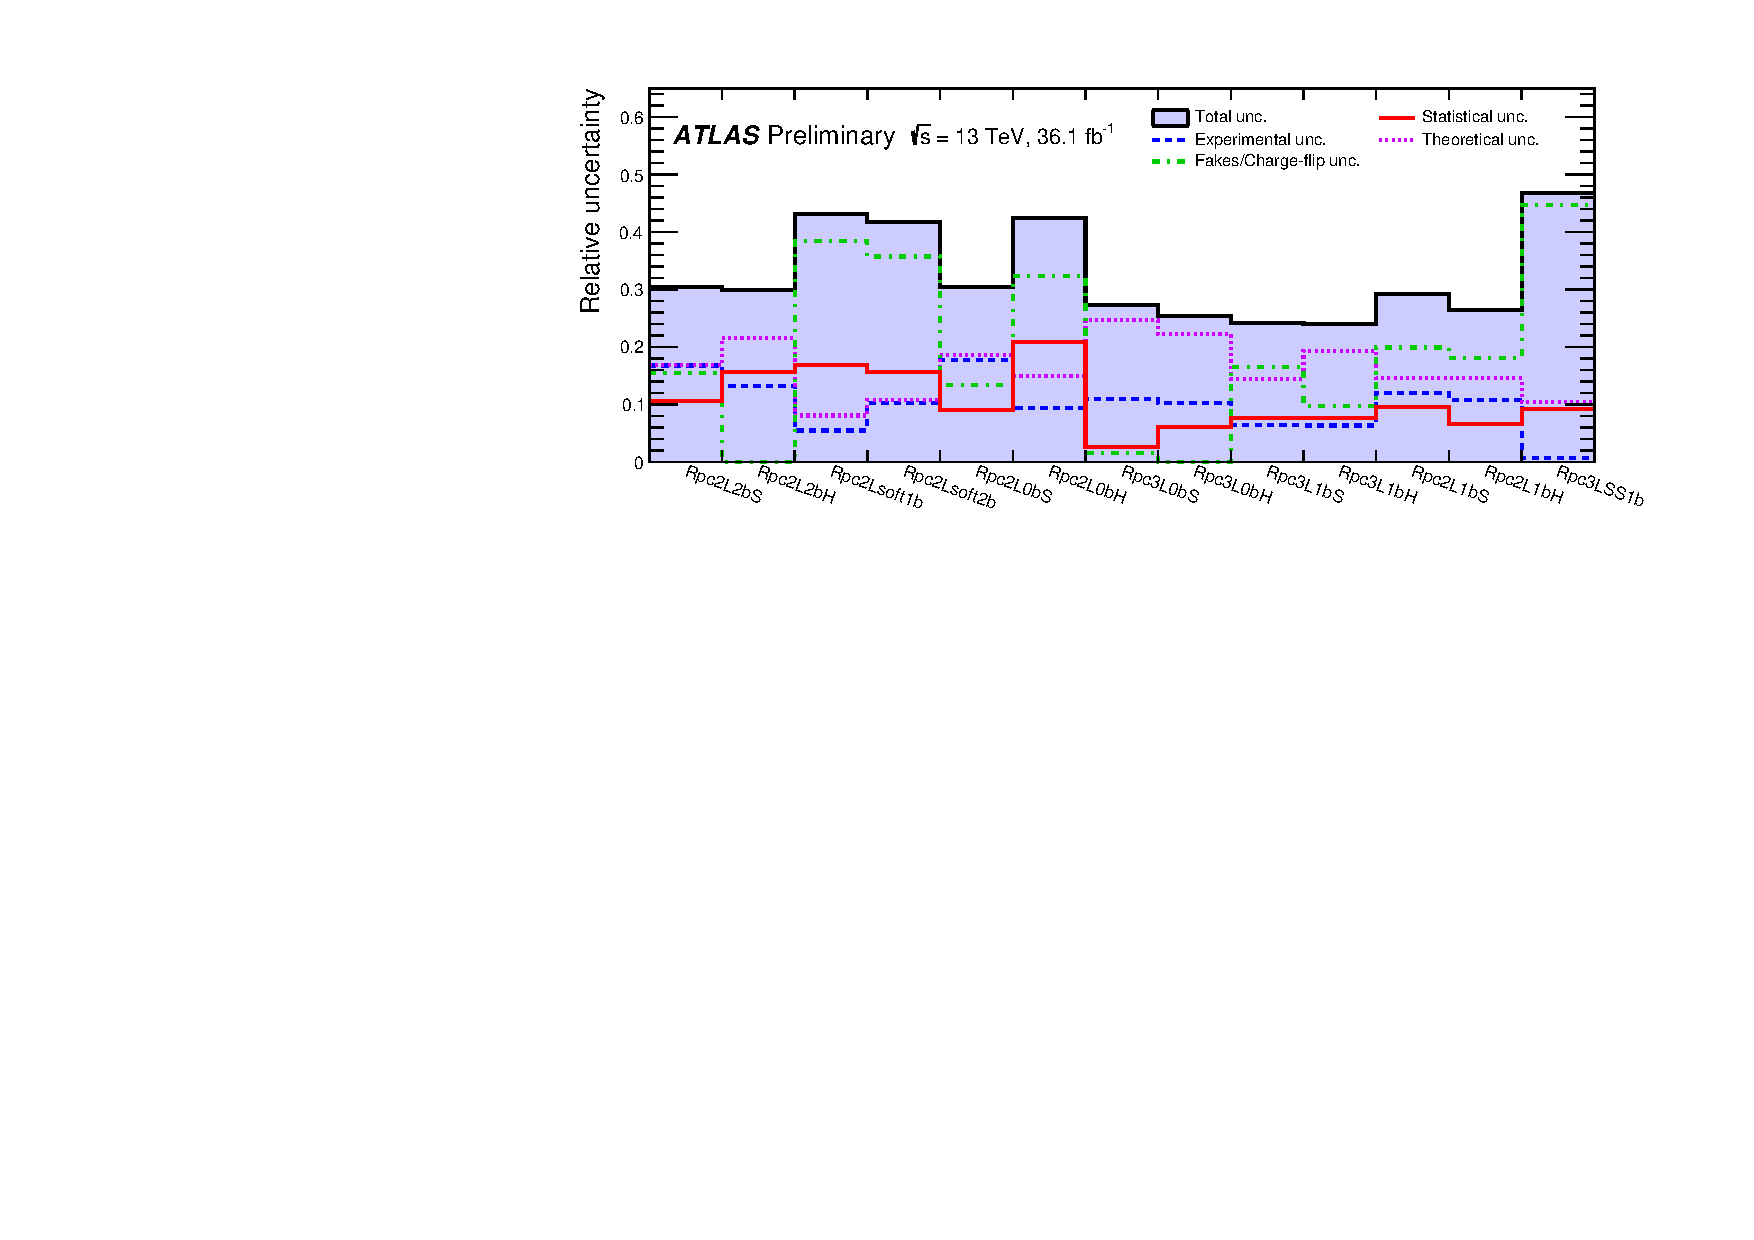
\includegraphics[width=\textwidth]{SystematicsSummary}\caption{}\label{fig:Results_SystSum}\end{subfigure}
\end{center}
\caption{Comparison of (a) the observed and expected event yields in each signal region and (b) the relative uncertainties in the total 
background yield estimate. For the latter, ``statistical uncertainty'' corresponds to reducible and irreducible background 
statistical uncertainties. The background predictions correspond to those presented in Table~\ref{tab:SR_yields} and the 
rare category is explained in the text. } 
\label{fig:PlotSR}
\end{figure}


\begin{table}
\scriptsize
%\small
\begin{center}
\vspace*{-0.035\textwidth}
\resizebox{1.\textwidth}{!}{
\begin{tabular}{|l|c|c|c|c|c|c|}
\hline
Signal Region                  & \textbf{Rpc2L2bS} & \textbf{Rpc2L2bH}    & \textbf{Rpc2Lsoft1b} &\textbf{Rpc2Lsoft2b}& \textbf{Rpc2L0bS} & \textbf{Rpc2L0bH}\\
\hline
\hline
$\ttbar W$, $\ttbar Z\gamma^*$ & $1.6\pm0.4$       & $0.44\pm0.14$     & $1.3\pm0.4$       & $1.21\pm0.33$       & $0.82\pm0.31$       & $0.20\pm0.10$  \\
$\ttbar H$                     & $0.43\pm0.25$     & $0.10\pm0.06$     & $0.45\pm0.24$     & $0.36\pm0.21$       & $0.27\pm0.15$       & $0.08\pm0.07$   \\
4$t$                           & $0.26\pm0.13$     & $0.18\pm0.09$     & $0.09\pm0.05$     & $0.21\pm0.11$       & $0.01\pm0.01$       & $0.02\pm0.02$   \\
Diboson                        & $0.10\pm0.10$     & $0.04\pm0.02$     & $0.17\pm0.09$     & $0.05\pm0.03$       & $3.1\pm1.4$         & $1.0\pm0.5$   \\
Rare                           & $0.33\pm0.18$     & $0.15\pm0.09$     & $0.18\pm0.10$     & $0.17\pm0.10$       & $0.19\pm0.11$       & $0.17\pm0.10$   \\
Fake/non-prompt leptons        & $0.5\pm0.6$       & $0.15\pm0.15$     & $3.5\pm2.4$       & $1.7\pm1.5$         & $1.6\pm1.0$         & $0.9\pm0.9$   \\
Charge-flip                    & $0.10\pm0.01$     & $0.02\pm0.01$     & $0.08\pm0.02$     & $0.08\pm0.02$       & $0.05\pm0.01$       & $0.01\pm0.01$   \\ 
\hline
Total Background               & $3.3\pm1.0$       & $1.08\pm0.32$     & $5.8\pm2.5$       & $3.8 \pm1.6$        & $6.0\pm1.8$         & $2.4\pm1.0$   \\
\hline
Observed                       & $3$               & $0$               & $4$               & $5$                 & $7$                 & $3$   \\
\hline\hline
$S_{\textrm{obs}}^{95}$        & \ral{$5.5$}               & \ral{$3.6$}               & \ral{$6.3$}               & \ral{$7.7$}               & \ral{$8.3$}               & \ral{$6.1$}  \\
$S_{\textrm{exp}}^{95}$        & \ral{$5.6_{-1.5}^{+2.2}$} & \ral{$3.9_{-0.4}^{+1.4}$} & \ral{$7.1_{-1.5}^{+2.5}$} & \ral{$6.2_{-1.5}^{+2.6}$} & \ral{$7.5_{-1.8}^{+2.6}$} & \ral{$5.3_{-1.3}^{+2.1}$} \\
$\sigma_{\textrm{vis}}$ [fb]   & \ral{$0.15$}              & \ral{$0.10$}              & \ral{$0.17$}              & \ral{$0.21$}              & \ral{$0.23$}              & \ral{$0.17$}  \\
$p_{0}$ ($\textrm{Z}$)         & \ral{$0.71$ (--)}         & \ral{$0.91$ (--)}         & \ral{$0.69$ (--)}         & \ral{$0.30\ (0.5\sigma)$} & \ral{$0.36\ (0.4\sigma)$} & \ral{$0.35\ (0.4\sigma)$}  \\
\hline 
\end{tabular}}

\vspace*{1cm}
\resizebox{1.\textwidth}{!}{
\begin{tabular}{|l|c|c|c|c|c|c|c|}
\hline
Signal Region 		& \textbf{Rpc3L0bS } 	& \textbf{Rpc3L0bH } 	& \textbf{Rpc3L1bS } 	& \textbf{Rpc3L1bH } 	& \textbf{Rpc2L1bS } 	& \textbf{Rpc2L1bH } 	& \textbf{Rpc3LSS1b }\\
\hline
\hline
$\ttbar W$, $\ttbar Z\gamma^*$   & $0.98\pm0.25$       	& $0.18\pm0.08$       	& $7.1\pm1.1$       	& $1.54\pm0.28$       	& $4.0\pm1.0$ 		& $4.0\pm0.9$	  	&  --     		\\
$\ttbar H$              & $0.12\pm0.08$       	& $0.03\pm0.02$       	& $1.4\pm0.7$       	& $0.25\pm0.14$       	& $1.3\pm0.7$ 		& $1.0\pm0.6$	  	& $0.22\pm0.12$    	\\
4$t$	   		& $0.02\pm0.01$	  & $0.01\pm0.01$	  & $0.7\pm0.4$ 	  & $0.28\pm0.15$	  & $0.34\pm0.17$	  & $0.54\pm0.28$	  &  -- 		  \\
Diboson                  & $8.9\pm2.9$       	& $2.6\pm0.8$       	& $1.4\pm0.5$       	& $0.48\pm0.17$       	& $0.5\pm0.3$ 		& $0.7\pm0.3$ 		&  --     		\\
Rare                     & $0.7\pm0.4$       	& $0.29\pm0.16$       	& $2.5\pm1.3$       	& $0.9\pm0.5$       	& $0.9\pm0.5$		& $1.0\pm0.6$		& $0.12\pm0.07$    	\\
Fake/non-prompt leptons  & $0.23\pm0.23$       	& $0.15\pm0.15$       	& $4.2\pm3.1$       	& $0.5\pm0.5$       	& $2.5\pm2.2$ 		& $2.3\pm1.9$  		& $0.9\pm0.7$    	\\
Charge-flip              &  --   		&  --    		&  --    		&  --     		& $0.25\pm0.04$ 	& $0.25\pm0.05$  	& $0.39\pm0.08$		\\	
\hline
Total Background         & $11.0\pm3.0\hpO$	       & $3.3\pm0.8$       	& $17\pm4\hpO$       	& $3.9\pm0.9$       	& $9.8\pm2.9$ 		& $9.8\pm2.6$  		& $1.6\pm0.8$	   	\\
\hline
Observed                 & $9$       		& $3$       		& $20$		       	& $4$       		& $14$  		&  $13$    		&  $1$			  \\
\hline\hline
$S_{\textrm{obs}}^{95}$       & \ral{$8.3$}	  	& $5.4$	   		& \ral{$14.7$}	    	& \ral{$6.1$}	     		& \ral{$13.7$}  		& \ral{$12.4$}   		& \ral{$3.9$}     		\\
$S_{\textrm{exp}}^{95}$       & \ral{$9.3_{-2.3}^{+3.1}$}	& \ral{$5.5_{-1.5}^{+2.2}$}	& \ral{$12.6_{-3.4}^{+5.1}$} 	& \ral{$5.9_{-1.8}^{+2.2}$}	& \ral{$10.0_{-2.6}^{+3.7}$}	& \ral{$9.7_{-2.6}^{+3.4}$}   & \ral{$4.0_{-0.3}^{+1.8}$}    \\
$\sigma_{\textrm{vis}}$ [fb] & \ral{$0.23$}		& \ral{$0.15$}  		& \ral{$0.41$}      		& \ral{$0.17$}      		& \ral{$0.38$}  		& \ral{$0.34$}   		& \ral{$0.11$}     		\\
$p_{0}$ ($\textrm{Z}$)        & \ral{$0.72$ (--)}  	& \ral{$0.85$ (--)}  		& \ral{$0.32\ (0.5\sigma)$}  & \ral{$0.46\ (0.1\sigma)$}  	& \ral{$0.17\ (1.0\sigma)$}  	& \ral{$0.21\ (0.8\sigma)$}	& \ral{$0.56$ (--)}	\\
\hline 
\end{tabular}}

\vspace*{1cm}

\vspace*{-0.01\textheight}\caption{Numbers of events observed in the signal regions compared with the expected backgrounds. 
The rare category is defined in the text. Background categories with yields shown as a ``--'' 
do not contribute to a given region (e.g. charge flips in three-lepton regions) or their estimates are below 0.01. 
The 95\% confidence level (CL) upper limits are shown on the observed and expected numbers of BSM events, $S_{\textrm{obs}}^{95}$ and $S_{\textrm{exp}}^{95}$ 
(as well as the $\pm 1\sigma$ excursions from the expected limit), respectively. The 95\% CL upper limits on the visible cross-section 
($\sigma_{\textrm{vis}}$) are also given. Finally the $p$-values ($p_{0}$) give the probabilities of the observations being consistent 
with the estimated backgrounds. The number of equivalent Gaussian standard deviations ($Z$) is also shown when $p_{0}<0.5$.}
\label{tab:SR_yields}
\end{center}
\end{table}

Figure~\ref{fig:Results_SystSum} summarizes the contributions from the different sources of systematic uncertainty 
to the total SM background predictions in the signal regions. The uncertainties amount to 25--45\% of the 
total background depending on the signal region, dominated by systematic uncertainties coming from the reducible background or the theory. 
The breakdown of the systematic uncertainties for each signal region is given in Table~\ref{tab:res.sys.break}


\begin{table}
\scriptsize
%\small
\begin{center}
\vspace*{-0.035\textwidth}
\resizebox{1.\textwidth}{!}{
\begin{tabular}{|l|c|c|c|c|c|c|}
\hline
Signal Region                  & \textbf{Rpc2L2bS} & \textbf{Rpc2L2bH}    & \textbf{Rpc2Lsoft1b} &\textbf{Rpc2Lsoft2b}& \textbf{Rpc2L0bS} & \textbf{Rpc2L0bH}\\
\hline
\hline
Total background expectation    &    $3.35 $    &   $1.08 $    &    $5.78 $    &    $3.80 $    &    $6.02 $    &    $2.35 $    \\
\hline
Total statistical    &    $10.56 \%$    &   $15.67 \%$    &    $16.93 \%$    &    $15.61 \%$    &    $9.08 \%$    &    $20.87 \%$    \\
Total background systematic    &    $30.41 \%$    &   $29.97 \%$    &    $43.10 \%$    &    $41.79 \%$    &    $30.51 \%$    &    $42.39 \%$    \\
\hline\hline
Fake/non-prompt    &    $15.46 \%$    &   $0.00 \%$    &    $38.39 \%$    &    $35.75 \%$    &    $13.46 \%$    &    $32.31 \%$    \\
Charge-flip    &    $0.06 \%$    &   $0.00 \%$    &    $0.35 \%$    &    $0.53 \%$    &    $0.17 \%$    &    $0.00 \%$    \\
\hline
Jet Energy Scale    &    $15.19 \%$    &   $11.37 \%$    &    $5.27 \%$    &    $9.28 \%$    &    $17.28 \%$    &    $8.11 \%$    \\
Other Jet Unc.    &    $2.09 \%$    &   $2.71 \%$    &    $0.80 \%$    &    $0.99 \%$    &    $2.31 \%$    &    $3.42 \%$    \\
Flavor Tagging    &    $6.27 \%$    &   $5.55 \%$    &    $0.81 \%$    &    $3.96 \%$    &    $3.33 \%$    &    $3.27 \%$    \\
Electrons    &    $1.20 \%$    &   $1.72 \%$    &    $0.51 \%$    &    $0.51 \%$    &    $0.76 \%$    &    $0.74 \%$    \\
Muons    &    $0.90 \%$    &   $1.39 \%$    &    $0.35 \%$    &    $0.51 \%$    &    $0.83 \%$    &    $0.93 \%$    \\
Missing transverse momentum    &    $2.24 \%$    &   $1.68 \%$    &    $0.85 \%$    &    $1.50 \%$    &    $0.65 \%$    &    $0.54 \%$    \\
\hline
Diboson Th. Unc.    &    $1.07 \%$    &   $1.39 \%$    &    $1.07 \%$    &    $0.50 \%$    &    $17.68 \%$    &    $13.54 \%$    \\
ttV Th. Unc.    &    $7.33 \%$    &   $8.86 \%$    &    $5.01 \%$    &    $4.48 \%$    &    $4.06 \%$    &    $2.44 \%$    \\
Rare Th. Unc.    &    $15.18 \%$    &   $19.67 \%$    &    $6.28 \%$    &    $9.75 \%$    &    $3.89 \%$    &    $5.87 \%$    \\
PDF    &    $0.00 \%$    &   $0.00 \%$    &    $0.00 \%$    &    $0.00 \%$    &    $0.00 \%$    &    $0.00 \%$    \\
\hline 
\end{tabular}}

\vspace*{1cm}
\resizebox{1.\textwidth}{!}{
\begin{tabular}{|l|c|c|c|c|c|c|c|}
\hline
Signal Region 		& \textbf{Rpc3L0bS } 	& \textbf{Rpc3L0bH } 	& \textbf{Rpc3L1bS } 	& \textbf{Rpc3L1bH } 	& \textbf{Rpc2L1bS } 	& \textbf{Rpc2L1bH } 	& \textbf{Rpc3LSS1b }\\
\hline
\hline
       Total background expectation    &    $11.02 $    &   $3.31 $    &    $17.33 $    &    $3.90 $    &    $9.88 $    &    $9.75 $       &    $1.62 $     \\
        \hline
        Total statistical    &    $2.57 \%$    &   $6.05 \%$    &    $7.66 \%$    &    $7.70 \%$    &    $9.59 \%$    &    $6.65 \%$       &    $9.15 \%$     \\
        Total background systematic    &    $27.37 \%$    &   $25.40 \%$    &    $24.22 \%$    &    $24.02 \%$    &    $29.19 \%$    &    $26.52 \%$       &    $46.79 \%$     \\
        \hline\hline
        Fake/non-prompt    &    $1.63 \%$    &   $0.00 \%$    &    $16.50 \%$    &    $9.73 \%$    &    $19.93 \%$    &    $18.05 \%$       &    $44.45 \%$     \\
        Charge-flip    &    $0.00 \%$    &   $0.00 \%$    &    $0.00 \%$    &    $0.00 \%$    &    $0.40 \%$    &    $0.41 \%$       &    $4.32 \%$     \\
        \hline
        Jet Energy Scale    &    $9.78 \%$    &   $8.98 \%$    &    $5.54 \%$    &    $4.20 \%$    &    $11.71 \%$    &    $10.40 \%$       &    $0.02 \%$     \\
        Other Jet Unc.    &    $3.41 \%$    &   $2.55 \%$    &    $0.70 \%$    &    $2.30 \%$    &    $1.42 \%$    &    $1.46 \%$       &    $0.20 \%$     \\
        Flavor Tagging    &    $2.79 \%$    &   $2.93 \%$    &    $2.22 \%$    &    $2.82 \%$    &    $1.32 \%$    &    $1.38 \%$       &    $0.32 \%$     \\
        Electrons    &    $1.78 \%$    &   $2.16 \%$    &    $1.66 \%$    &    $2.47 \%$    &    $0.67 \%$    &    $0.89 \%$       &    $0.41 \%$     \\
        Muons    &    $1.73 \%$    &   $2.12 \%$    &    $1.25 \%$    &    $1.79 \%$    &    $0.80 \%$    &    $0.92 \%$       &    $0.41 \%$     \\
        Missing transverse momentum    &    $0.78 \%$    &   $0.53 \%$    &    $0.38 \%$    &    $0.59 \%$    &    $1.70 \%$    &    $1.06 \%$       &    $0.00 \%$     \\
        \hline
        Diboson Th. Unc.    &    $24.28 \%$    &   $21.58 \%$    &    $2.57 \%$    &    $3.78 \%$    &    $1.87 \%$    &    $2.50 \%$       &    $0.00 \%$     \\
        ttV Th. Unc.    &    $1.49 \%$    &   $1.76 \%$    &    $5.34 \%$    &    $5.56 \%$    &    $6.96 \%$    &    $5.72 \%$       &    $0.00 \%$     \\
        Rare Th. Unc.    &    $4.02 \%$    &   $5.02 \%$    &    $13.19 \%$    &    $18.11 \%$    &    $12.68 \%$    &    $13.16 \%$       &    $10.49 \%$     \\
        PDF    &    $0.00 \%$    &   $0.00 \%$    &    $0.00 \%$    &    $0.00 \%$    &    $0.00 \%$    &    $0.00 \%$       &    $0.00 \%$     \\
\hline 
\end{tabular}}

\vspace*{1cm}

\vspace*{-0.01\textheight}\caption{Breakdown of the dominant systematic uncertainties on background estimates in the various signal regions.
Note that the individual uncertainties can be correlated, and do not necessarily add up quadratically to 
the total background uncertainty. The percentages show the size of the uncertainty relative to the total expected background.}
\label{tab:res.sys.break}
\end{center}
\end{table}




\section{Statistical Interpretation}

In the absence of any significant deviation from the standard model predictions,
the results will be interpreted to 
 establish 95\% confidence intervals using the CL$_\mathrm{s}$ prescription~\cite{Read:2002hq} 
based on a profile-likelihood-ratio test~\cite{Cowan:2010js}
 described in Chapter~\ref{chap:stat}.
The interpretation will include upper limits on possible beyond the standard model contributions to the signal 
regions in a model independent way,
as well as exclusion limits on the masses of 
SUSY particles in the benchmark scenarios of Figure~\ref{fig:strategy.pheno.feynman}. 

\subsection{Model independent discovery and upper limits}

Table~\ref{tab:SR_yields} presents 95\% confidence level (CL) observed (expected) model-independent upper limits 
on the number of BSM events, $S_{\textrm{obs}}^{95}$ ($S_{\textrm{exp}}^{95}$), that may contribute to the signal regions. 
Normalizing these by the integrated luminosity $L$ of the data sample, they can be interpreted as upper limits on the visible 
BSM cross-section ($\sigma_{\textrm{vis}}$), defined as $\sigma_{\textrm{vis}}=\sigma_{\textrm{prod}}\times A \times\epsilon=S_{\textrm{obs}}^{95}/L$, where 
$\sigma_{\textrm{prod}}$ is the production cross-section, $A$ the acceptance and $\epsilon$ the reconstruction efficiency. The largest 
deviation of the data from the background prediction corresponds to an excess of 1.0 standard deviation in the Rpc2L1bS SR.


\subsection{Model dependent exclusion limits}

Exclusion limits at 95\% CL are set on the masses of the superpartners involved in the SUSY benchmark scenarios considered. 
Apart from the NUHM2 model, simplified models are used, corresponding to a single production mode and with 100\% branching ratio to a specific decay chain, 
with the masses of the SUSY particles not involved in the process set to very high values. 

In order to determine which signal region is used to set an exclusion limit 
on a particular model, the expected $CL_s$ value is computed for each signal 
region at a given point in the signal parameter space. The signal 
region with the smallest expected  $CL_s$ value (more disagreement with data 
under the signal hypothesis) is used to set an exclusion limit on the model.
An example on what signal region is performing best at a given model using the 
decay is shown in Figure~\ref{fig:res.best_gtt}.

\begin{figure}[htb!]
\centering
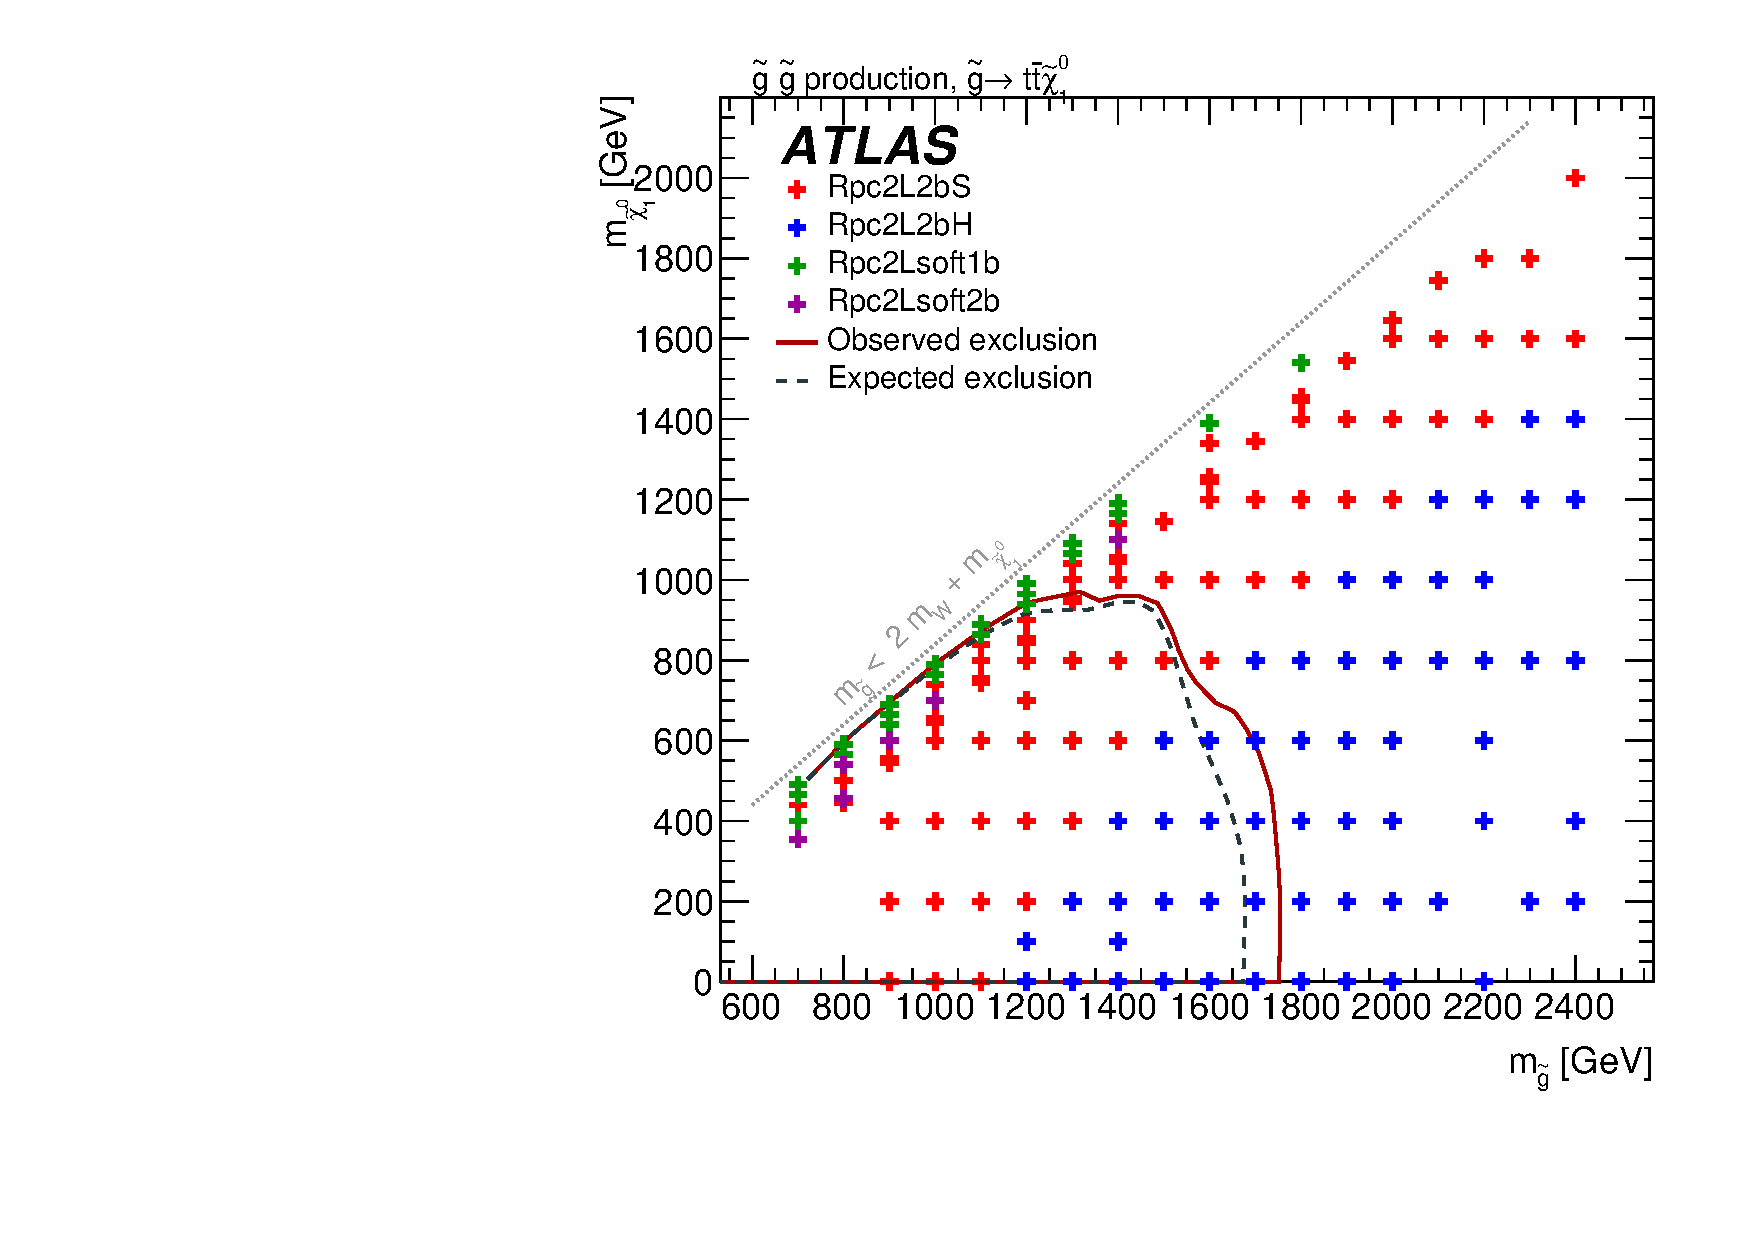
\includegraphics[width=.75\textwidth]{best_Rpc2L2b}
\caption{Illustration of the best expected signal region per signal grid point for the 
$\gluino \to t\bar t\neut$ (Fig.~\ref{fig:strategy.pheno.feynman_gtt}) model. 
This mapping is used for the final combined exclusion limits.}
\label{fig:res.best_gtt}
\end{figure}


Figures~\ref{fig:Results_Limits_RPC} and \ref{fig:Results_Limits_NUHM2} show the exclusion limits in all 
the models considered in Figure~\ref{fig:strategy.pheno.feynman} and the NUHM2 model. The assumptions about the decay chain considered for the different SUSY particles are 
stated above each figure. For each region of the signal parameter space, the SR with the best expected sensitivity is chosen.

Each one of the Figures~\ref{fig:Results_Limits_RPC} contain:
\begin{itemize}
\item Observed limit (thick solid red line): all uncertainties are included in the fit as nuisance 
parameters, with the exception of the theoretical signal uncertainties (PDF, scales) on the 
inclusive cross section.
\item Expected limit (less thick long-dashed black line): all uncertainties are included in the fit 
as nuisance parameters, with the exception of the theoretical signal uncertainties (PDF, scales) 
on the inclusive cross section. 
\item $\pm 1\sigma$ lines around the observed limit (thin dark-red dotted): re-run limit calculation
 while increasing or decreasing the signal cross section by the theoretical signal uncertainties 
  (PDF, scales).
\item $\pm 1\sigma$  band around expected limit (yellow band): represents the  $\pm 1\sigma$ 
uncertainty from the fit.
\end{itemize}

\begin{figure}[p]
\centering
\begin{subfigure}[t]{0.45\textwidth}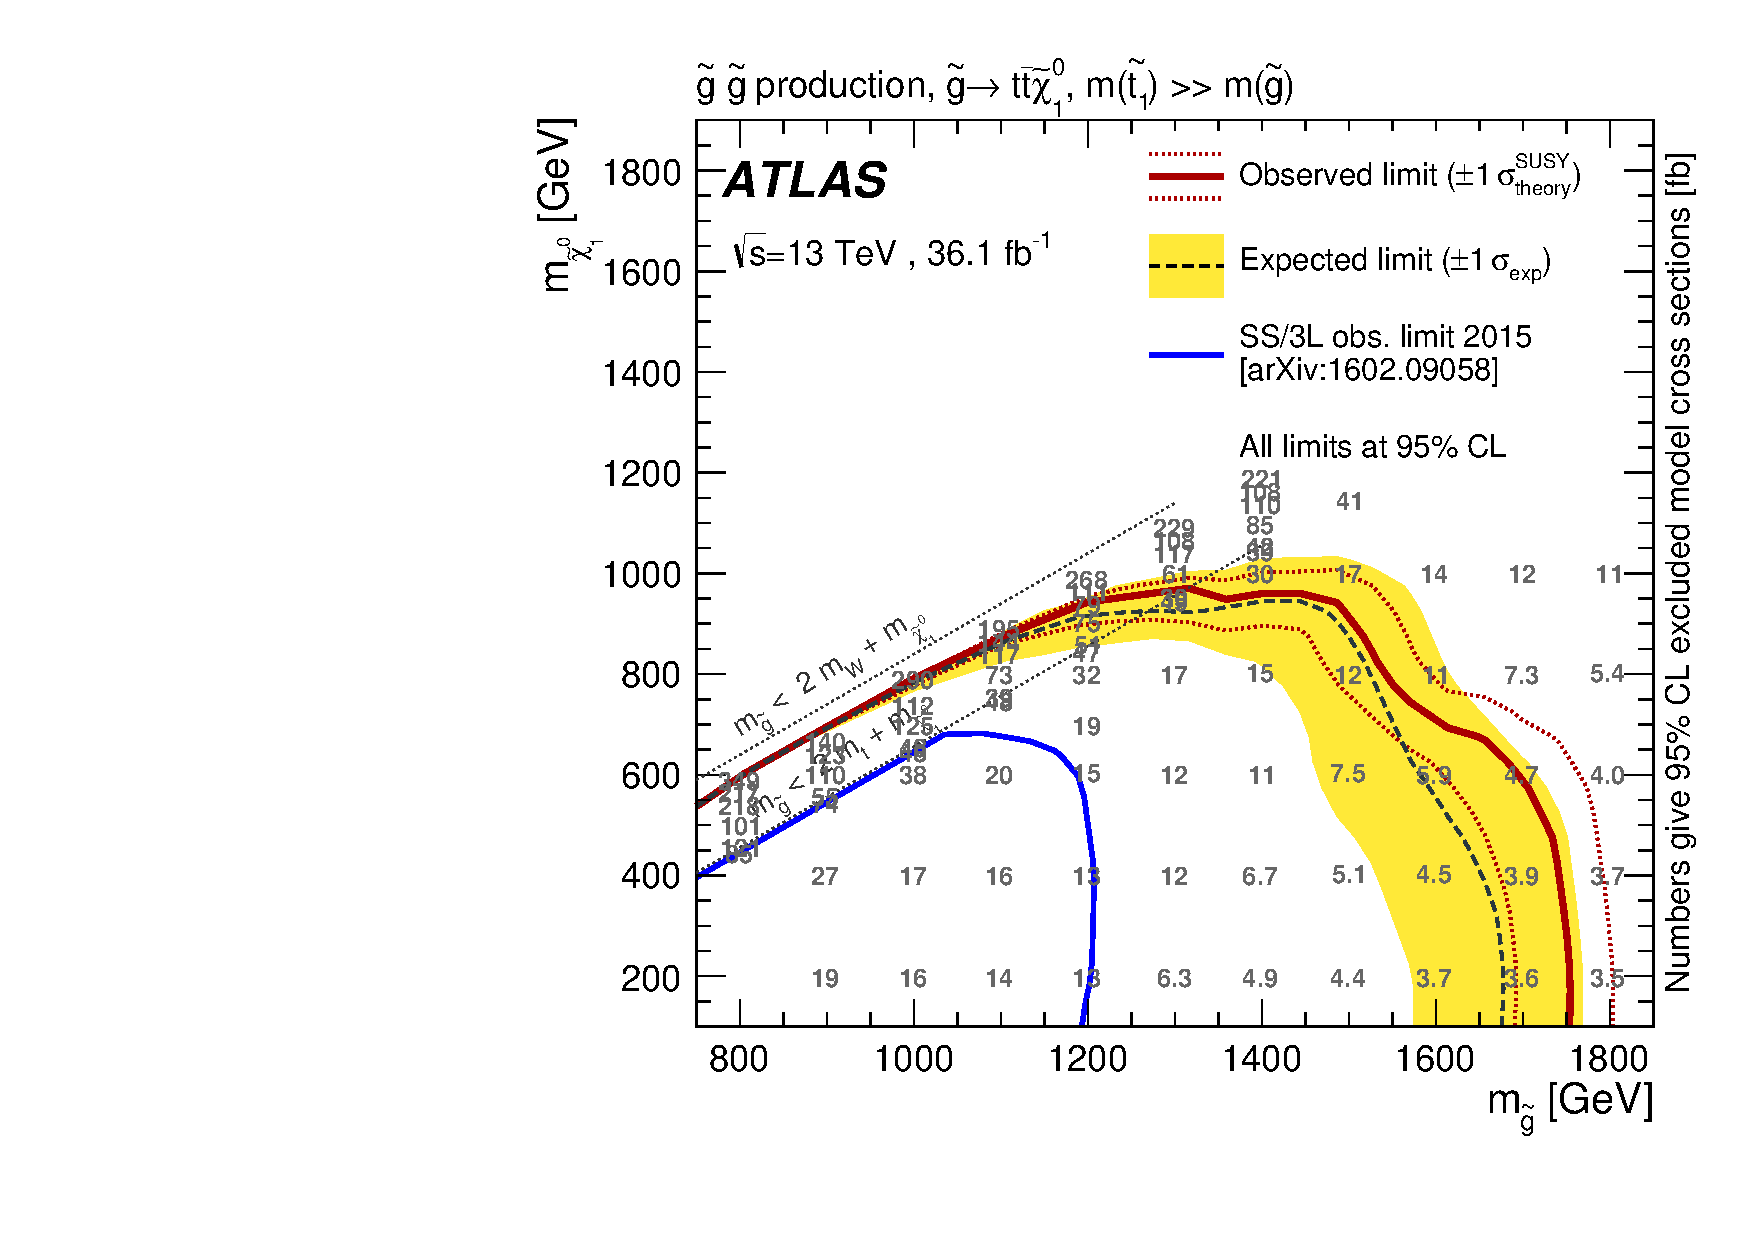
\includegraphics[width=\textwidth]{Gtt_SRbest}\caption{Rpc2L2bS/H, Rpc2Lsoft1b/2b}\label{fig:limits_feynman_gtt}\end{subfigure}
\begin{subfigure}[t]{0.45\textwidth}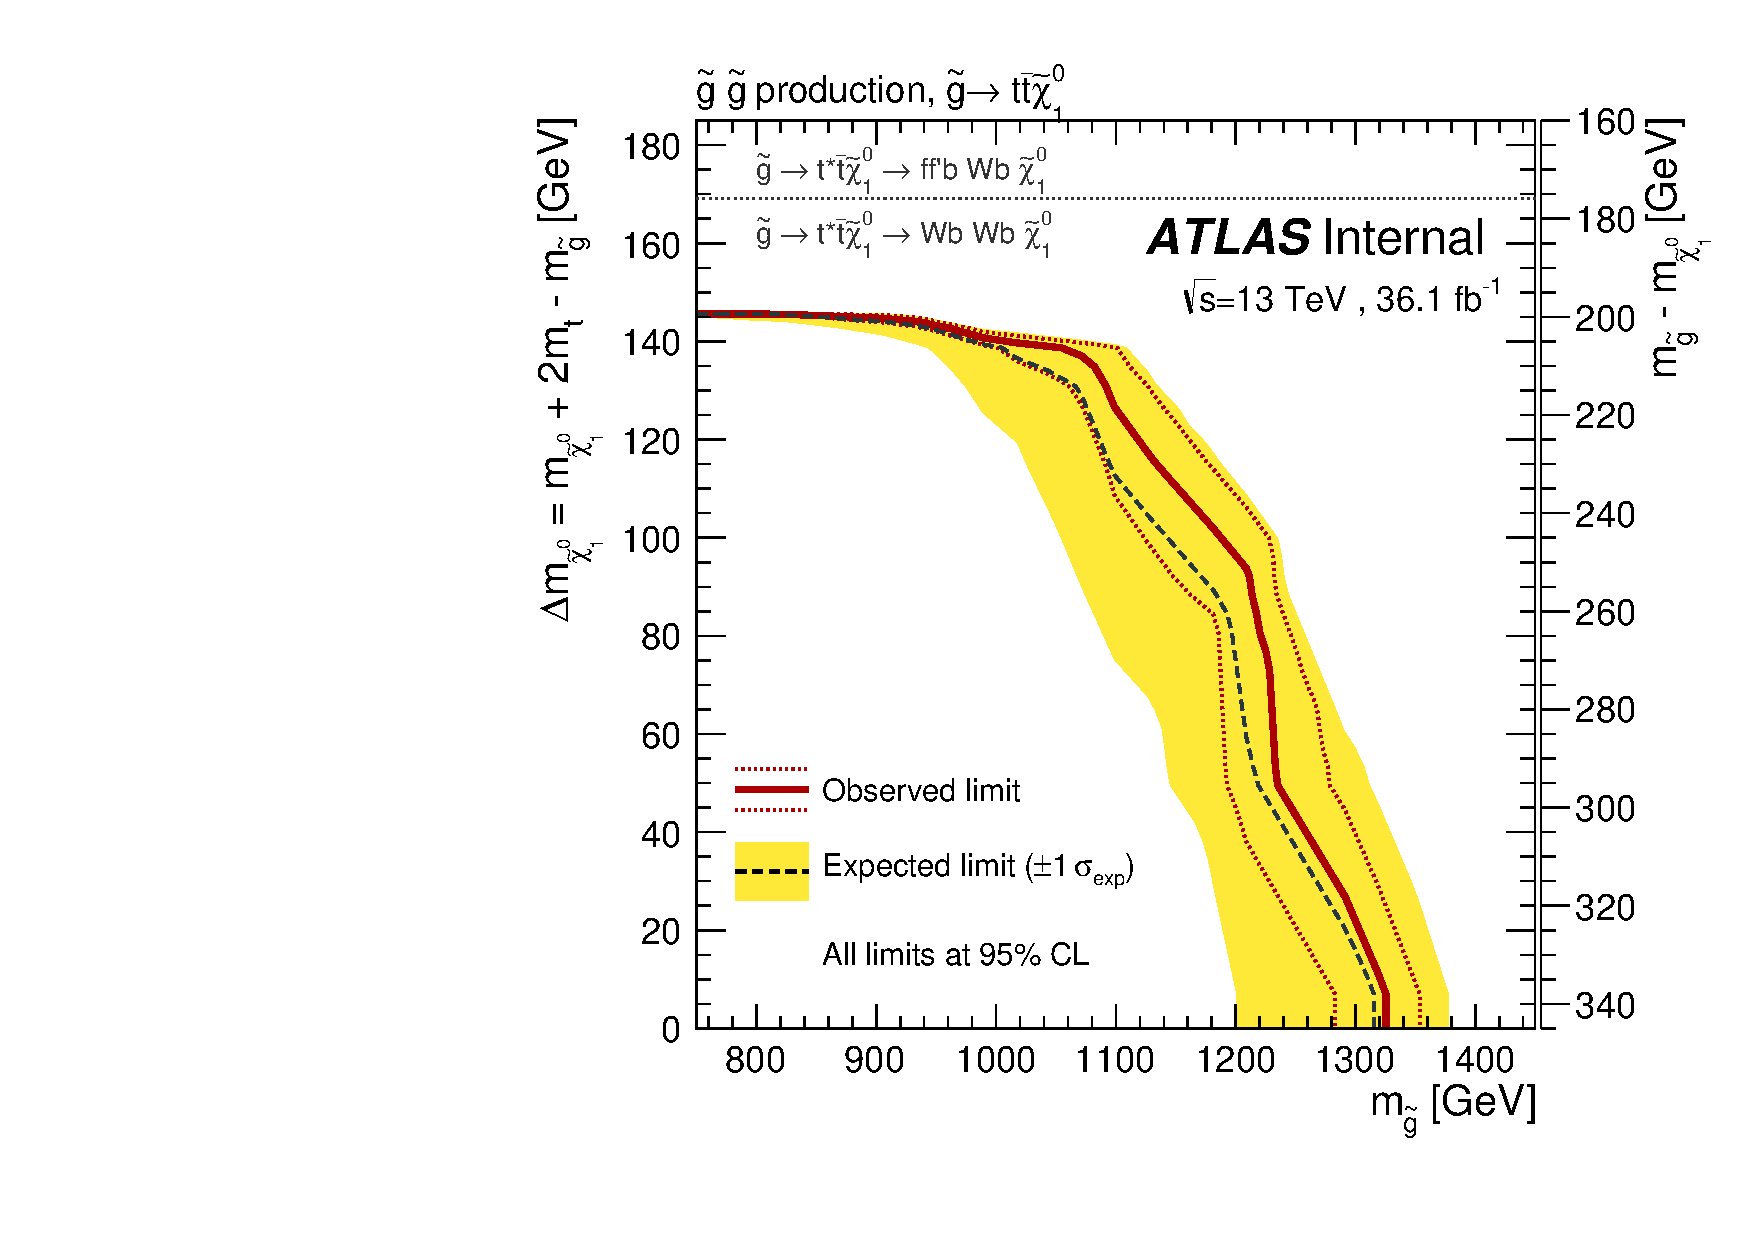
\includegraphics[width=\textwidth]{Gtt_above}\caption{Rpc2Lsoft1b, Rpc2Lsoft2b}\label{fig:limits_feynman_gttOffshell}\end{subfigure}
\caption{Observed and expected exclusion limits on the $\tilde{g}$ and \ninoone masses for (a) the model in Figure~\ref{fig:strategy.pheno.feynman_gtt} 
and (b) the model in Figure~\ref{fig:strategy.pheno.feynman_gttOffshell}. 
Figure (b) is a zoomed version of Figure (a) in the mass-parameter space where there is at least one top-quark off-shell decay.
All limits are computed at 95\% CL. The dotted lines around the observed
limit illustrate the change in the observed limit as the nominal signal cross-section is scaled up and down
by the theoretical uncertainty. The contours of the band around the expected 
limit are the $\pm$1$\sigma$ results, 
including all uncertainties except the theoretical ones in the signal cross-section. 
}
\label{fig:Results_Limits_RPC} 
\end{figure} 


\begin{figure}[p]
\centering
\begin{subfigure}[t]{0.45\textwidth}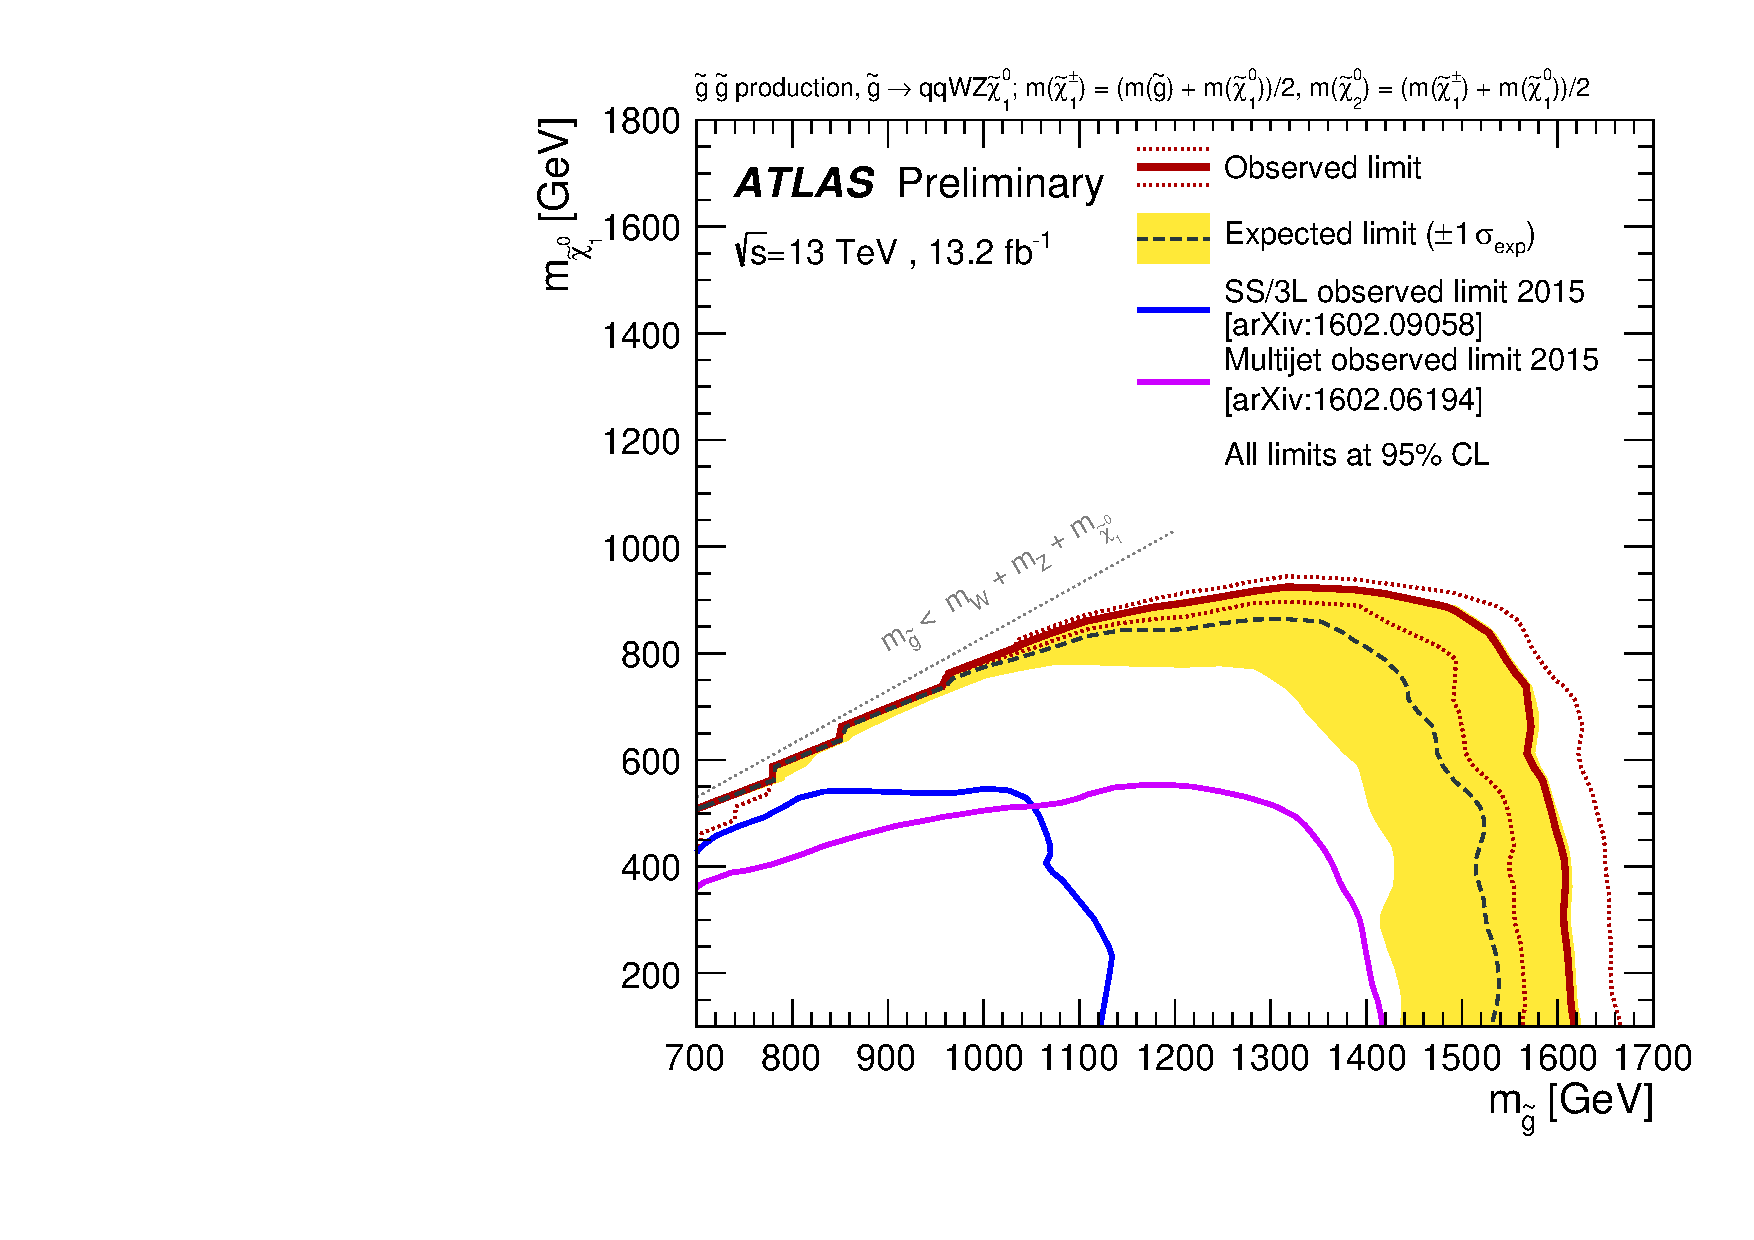
\includegraphics[width=\textwidth]{2stepWZ_SRbest}\caption{Rpc2L0bS, Rpc2L0bH}\label{fig:limits_feynman_gg2WZ}\end{subfigure}
\begin{subfigure}[t]{0.45\textwidth}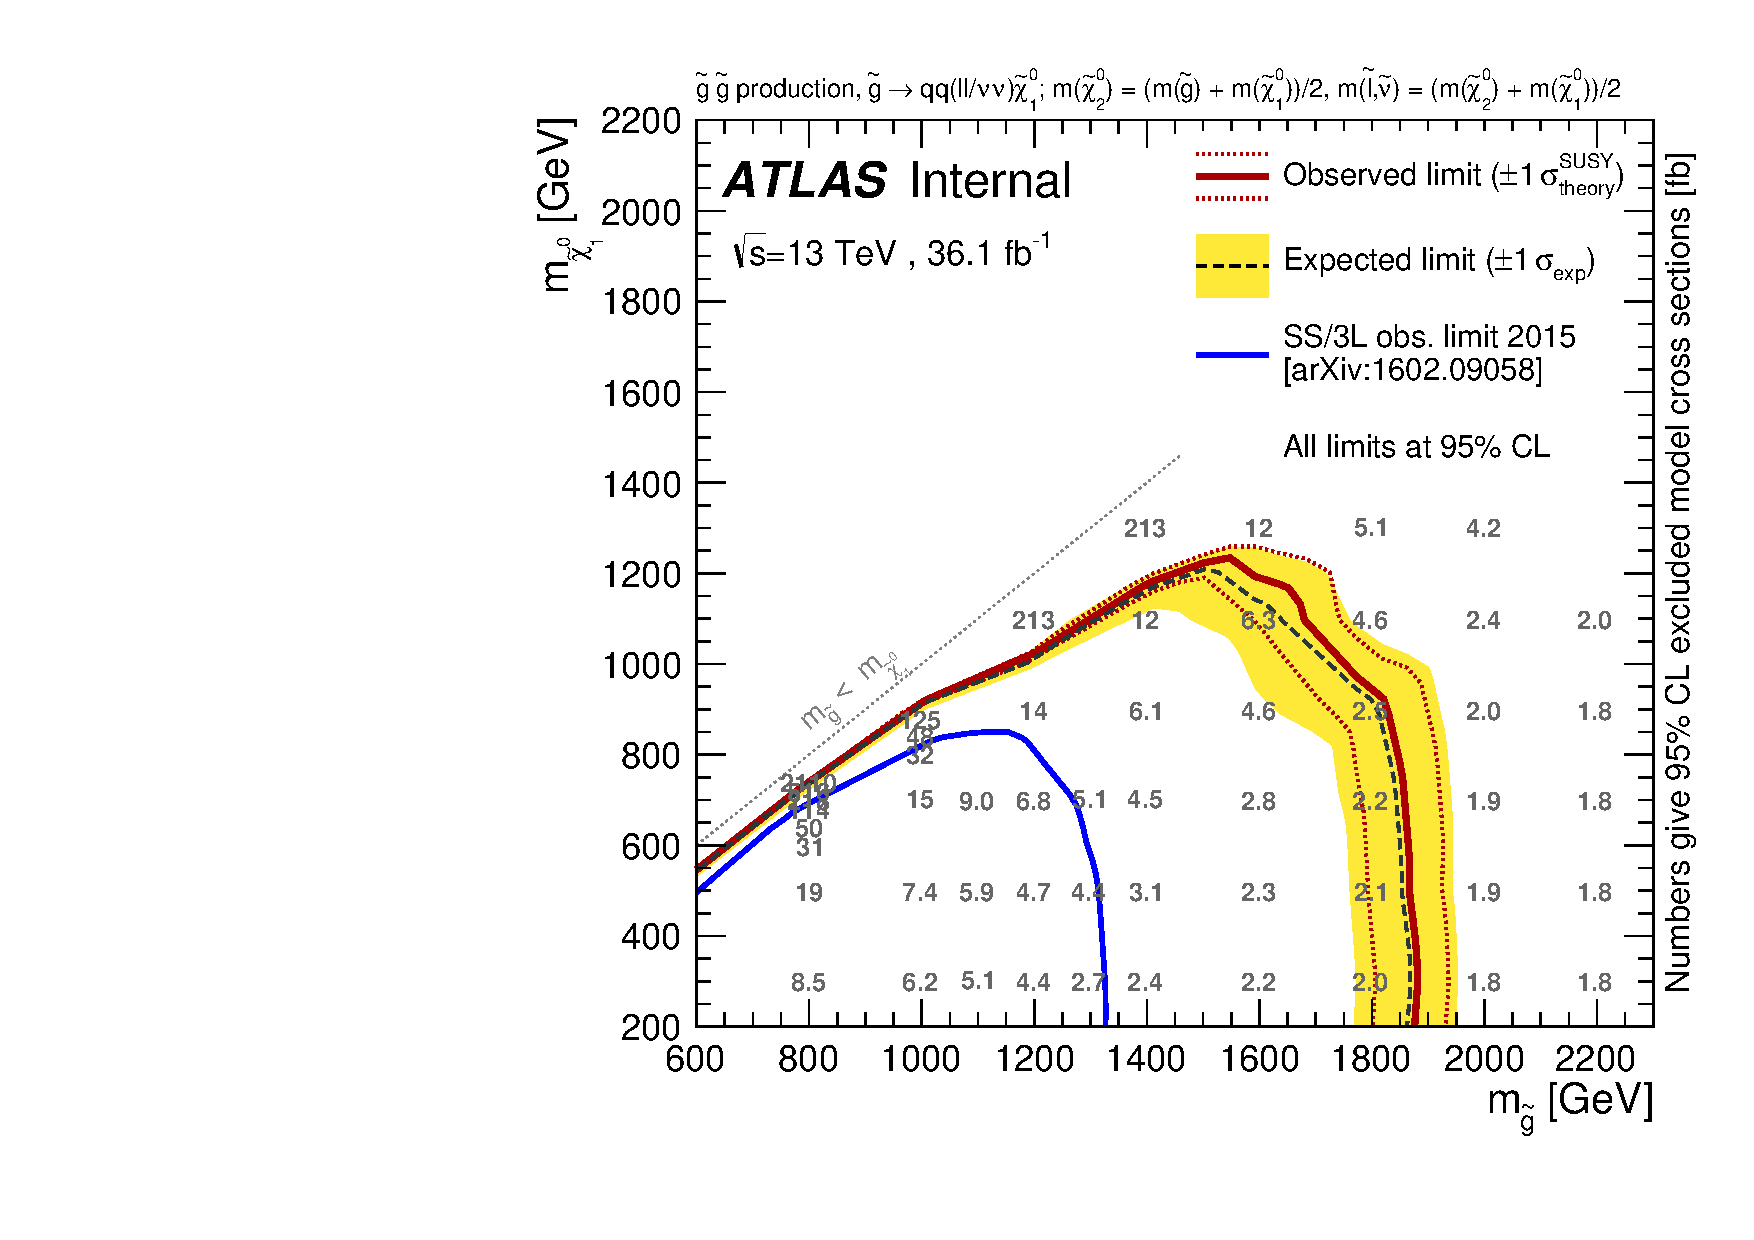
\includegraphics[width=\textwidth]{GSL_SRbest.pdf}\caption{Rpc3L0bS, Rpc3L0bH}\label{fig:limits_feynman_gg2sl}\end{subfigure}
\caption{Observed and expected exclusion limits on the $\tilde{g}$ and \ninoone masses 
for (a) the model in Figure~\ref{fig:strategy.pheno.feynman_gg2WZ} 
and (b) the model in Figure~\ref{fig:strategy.pheno.feynman_gg2sl}. 
All limits are computed at 95\% CL. The dotted lines around the observed
limit illustrate the change in the observed limit as the nominal signal cross-section is scaled up and down
by the theoretical uncertainty. The contours of the band around the expected 
limit are the $\pm$1$\sigma$ results,
including all uncertainties except the theoretical ones in the signal cross-section.}
\label{fig:Results_Limits_RPC} 
\end{figure} 

\begin{figure}[b]
\centering
\begin{subfigure}[t]{0.45\textwidth}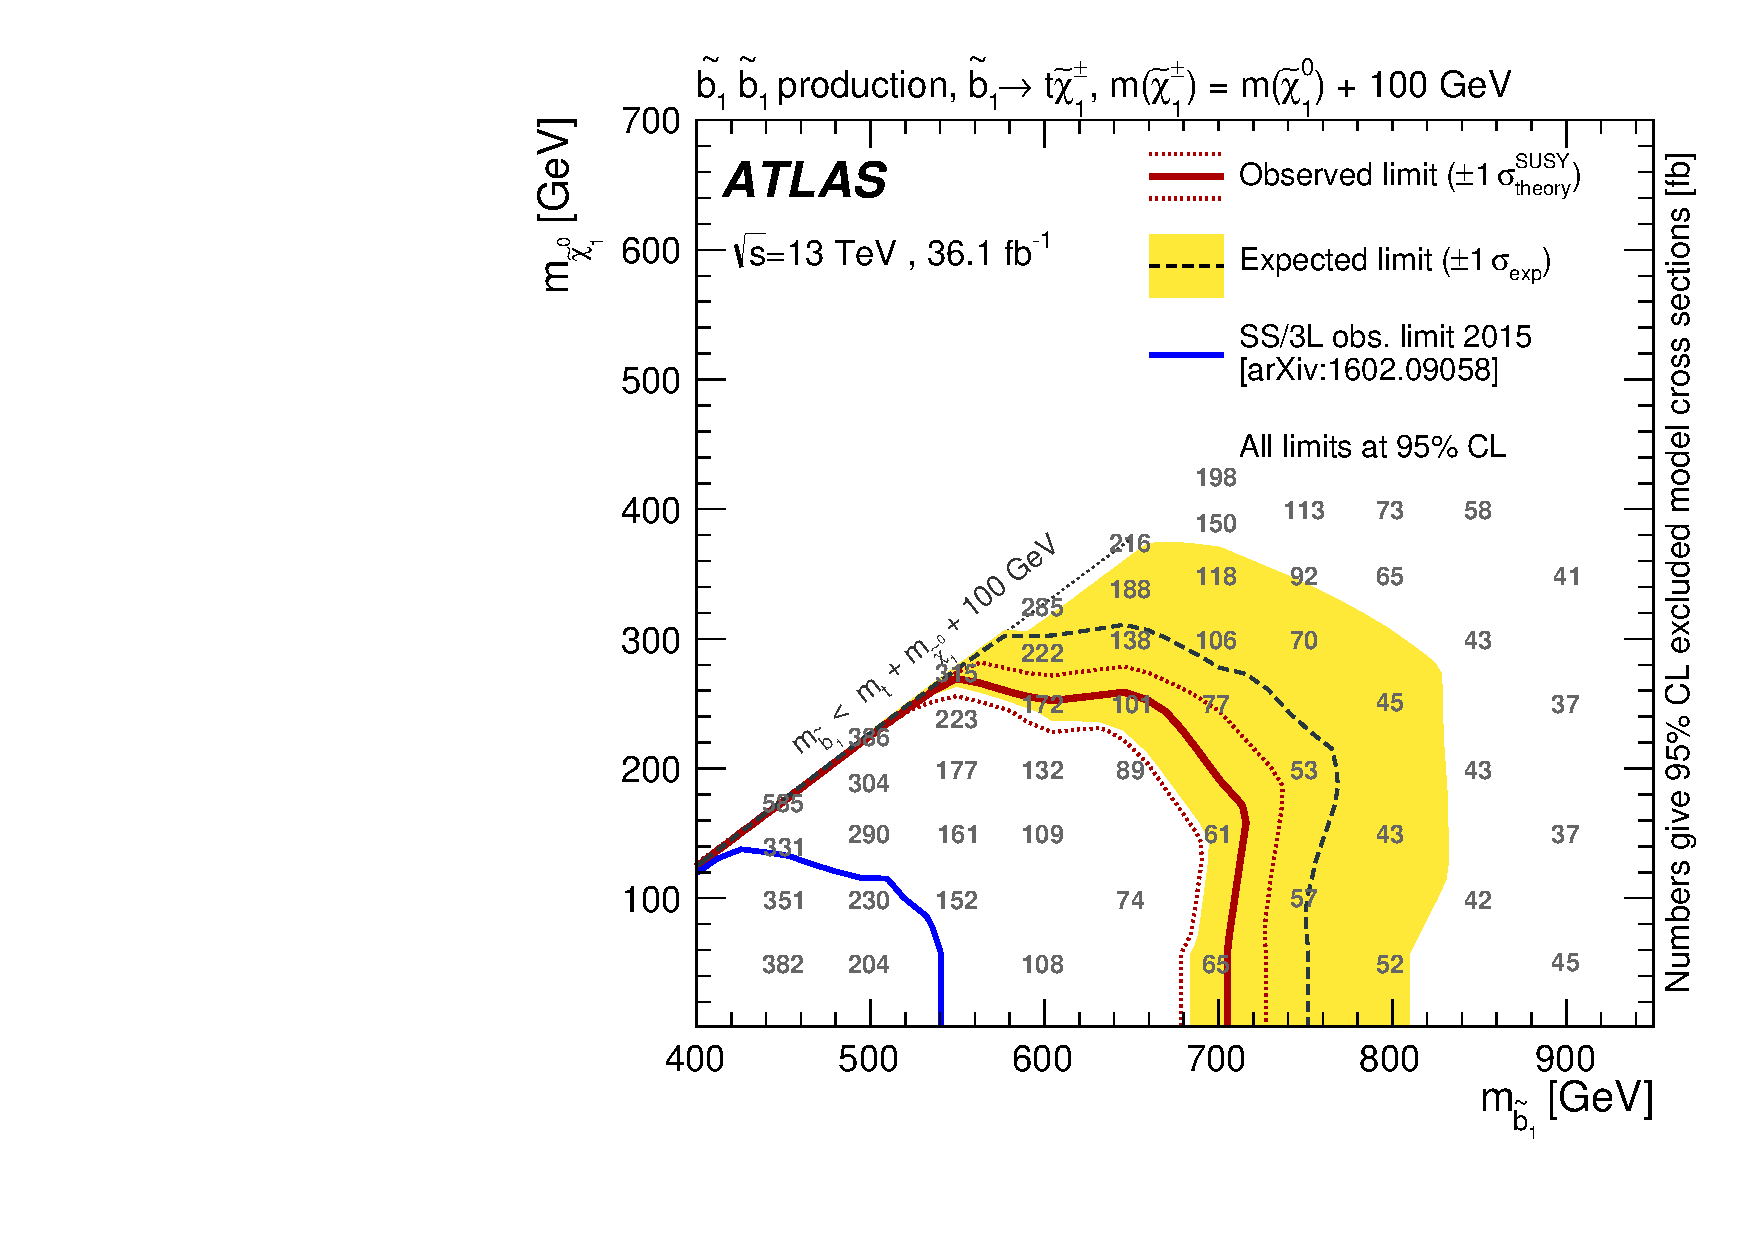
\includegraphics[width=\textwidth]{Btt_SRbest.pdf}\caption{Rpc2L1bS, Rpc2L1bH}\label{fig:limits_feynman_b1b1}\end{subfigure}
\begin{subfigure}[t]{0.45\textwidth}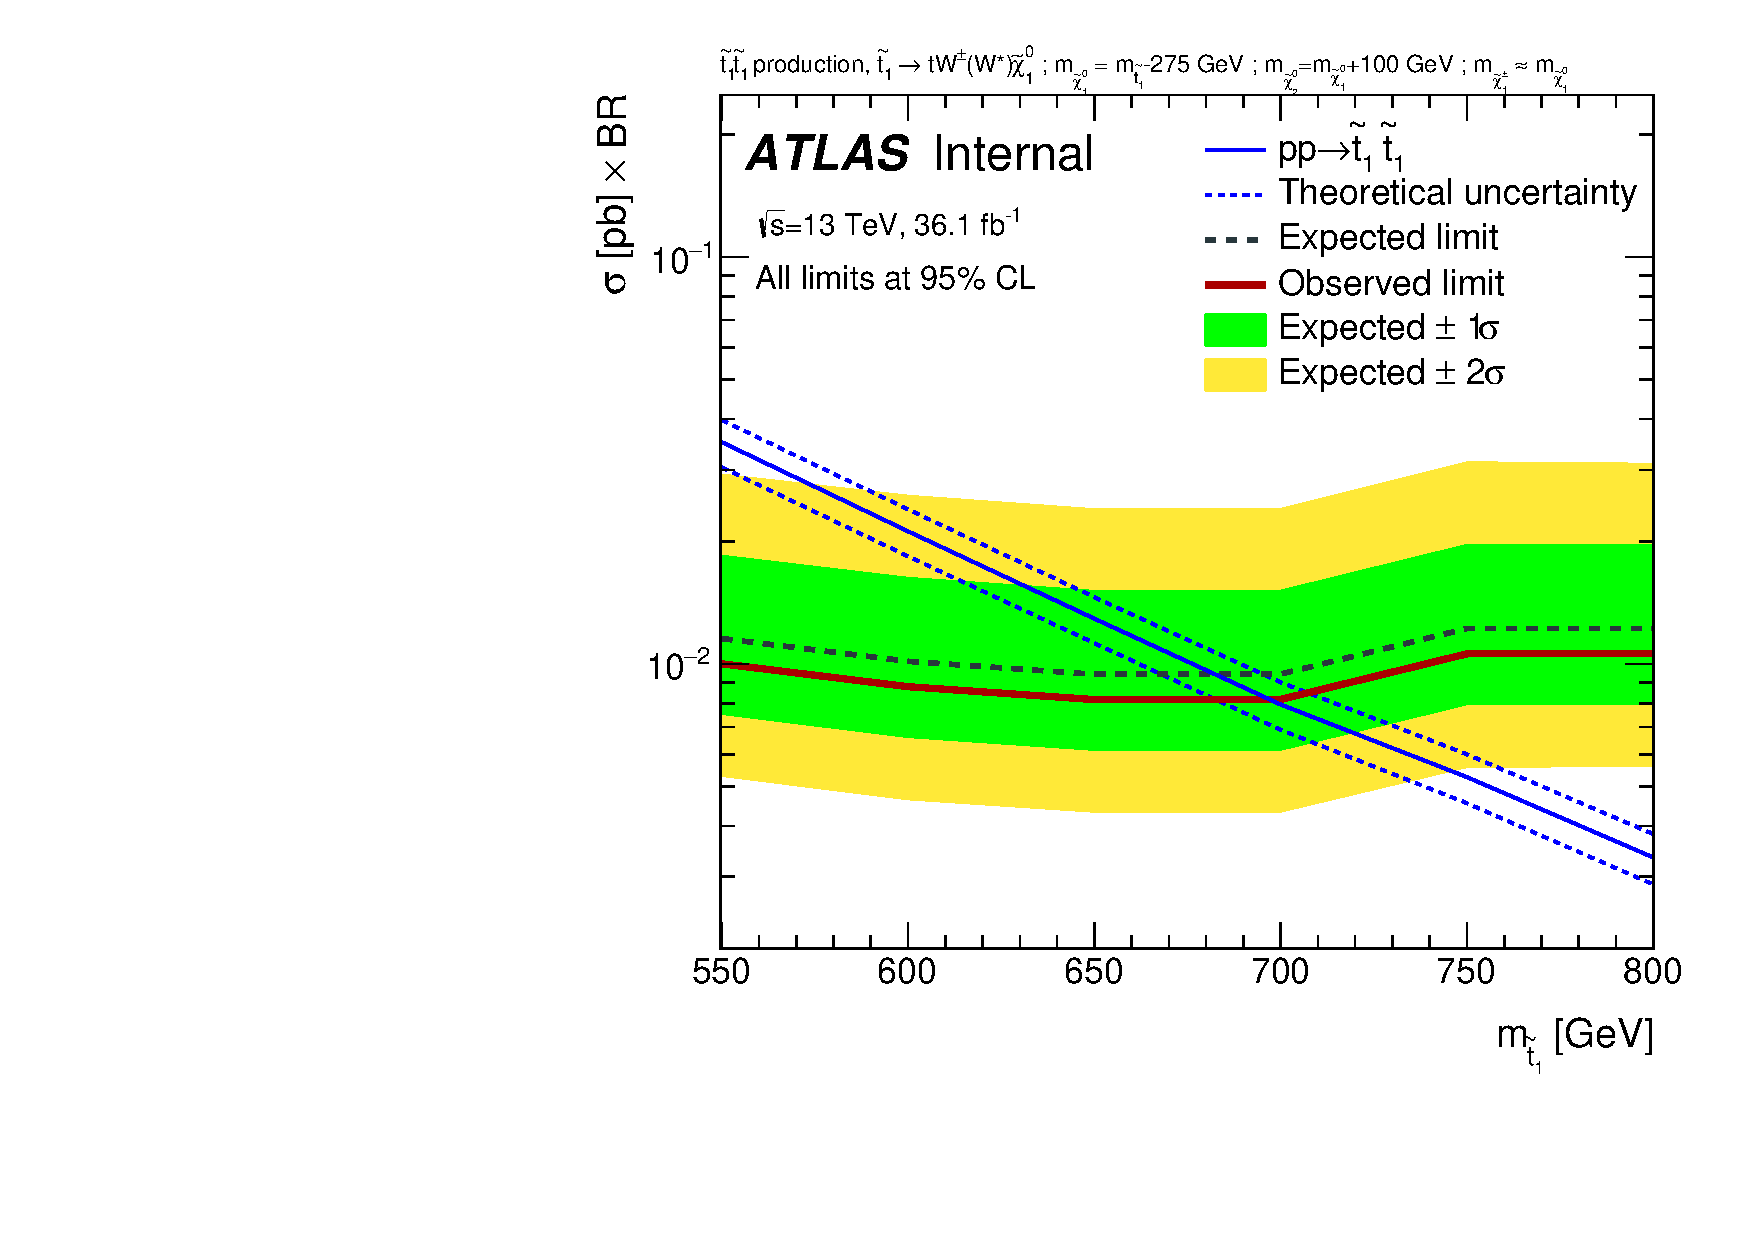
\includegraphics[width=\textwidth]{UL_TT2Step.pdf}\caption{Rpc3LSS1b}\label{fig:limits_feynman_t1t1}\end{subfigure}
\caption{
Observed and expected exclusion limits on the  \sbottomone, \stopone, and \ninoone masses 
for (a) the model in Figure~\ref{fig:strategy.pheno.feynman_b1b1}
and (b) the model in Figure~\ref{fig:strategy.pheno.feynman_t1t1}. 
The two models are complementary where the one-dimensional change in stop masses (b) is along the grayed diagonal in the sbottom plot (b).
All limits are computed at 95\% CL. The dotted lines around the observed
limit illustrate the change in the observed limit as the nominal signal cross-section is scaled up and down
by the theoretical uncertainty. The contours of the band around the expected 
limit are the $\pm$1$\sigma$ results  ($\pm$2$\sigma$ is also considered in (b)),
including all uncertainties except the theoretical ones in the signal cross-section.
}
\label{fig:Results_Limits_NUHM2} 
\end{figure} 

\begin{figure}[b]
\centering
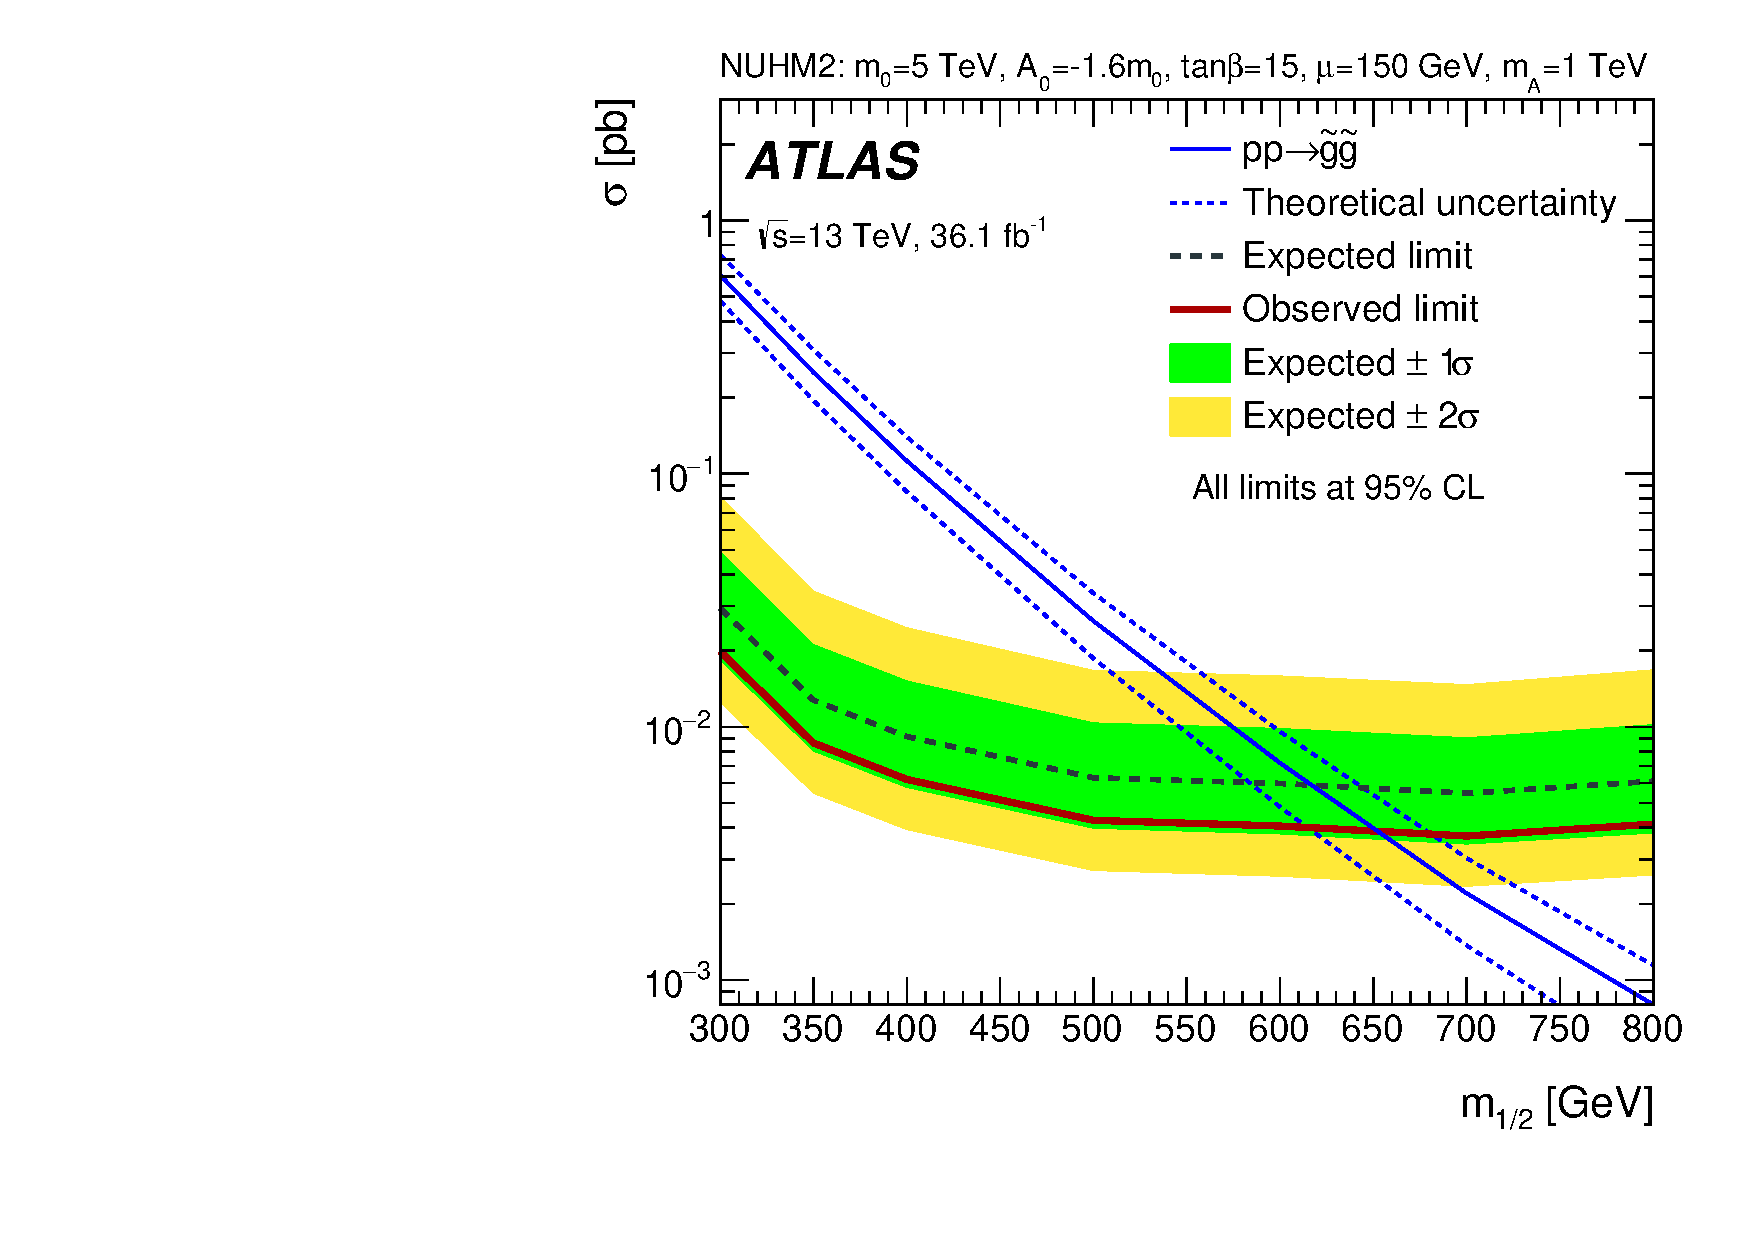
\includegraphics[width=0.7\textwidth]{UL_NUHM2}\label{fig:limits_feynman_nuhm2}
\caption{Observed and expected exclusion limits as a function of $m_{1/2}$ in the NUHM2 model~\cite{Ellis:2002iu,Ellis:2002wv}.
The signal region Rpc2L2bH is used to obtain the limits. 
The contours of the green (yellow) band around the expected limit are the $\pm$1$\sigma$ ($\pm$2$\sigma$) results, including all uncertainties. The limits are computed at 95\% CL.}
\label{fig:Results_Limits_NUHM2} 
\end{figure} 

The limits set are compared with the existing limits set by other ATLAS SUSY 
searches~\cite{paperSS3L,Aad:2016jxj}. For the models shown in Figure~\ref{fig:Results_Limits_RPC}, 
the mass limits on gluinos and bottom squarks are up to 400\GeV higher than the previous limits, reflecting the improvements 
in the signal region definitions as well as the increase in integrated luminosity. Gluinos with masses up to 1.75~\TeV~
are excluded in scenarios with a light $\ninoone$ in Figure~\ref{fig:limits_feynman_gtt}. This limit is extended to 1.87~\TeV~ when 
$\ninotwo$ and slepton masses are in between the gluino and the $\ninoone$ masses (Figure~\ref{fig:limits_feynman_gg2sl}). More generally, gluino masses 
below 1.57~\TeV~and bottom squarks with masses below 700~\GeV 
are excluded in models with a massless LSP. The ``compressed'' regions, where SUSY particle masses are close to each other, are also better covered 
and LSP masses up to 1200 and 250~\GeV~are excluded in the gluino and bottom squark pair-production models, respectively. Of particular
interest is the observed exclusion of models producing gluino pairs with an off-shell top quark in the decay (Figure~\ref{fig:strategy.pheno.feynman_gttOffshell}), 
see Figure~\ref{fig:limits_feynman_gtt}. In this case, models are excluded for mass differences between the gluino and neutralino of 205 GeV (only ~35 GeV
larger than the minimum mass difference for decays into two on-shell $W$ bosons and two $b$-quarks) for a gluino mass below 0.9
TeV. The Rpc3LSS1b SR allows the exclusion of top squarks with masses below 700~\GeV~when the top squark decays to a top quark and a cascade of electroweakinos 
$\ninotwo \to \chinoonepm W^{\mp} \to W^{*} W^{\mp} \ninoone$ (see Figure~\ref{fig:limits_feynman_t1t1} for the conditions 
on the sparticle masses).


Finally, in the NUHM2 model with low fine-tuning, values of the parameter $m_{1/2}$ below 615~\GeV~are excluded, 
corresponding to gluino masses below 1500~\GeV~(Figure~\ref{fig:Results_Limits_NUHM2}).
